\documentclass[a4paper,oneside]{book}
% ============ Import Library ============
% Apply template
% Using vietnamese
\usepackage[utf8]{vietnam}
\usepackage[vietnamese=nohyphenation]{hyphsubst}
\usepackage[vietnamese]{babel}
\usepackage[utf8]{inputenc}
% Some essential libs for math
\usepackage{amsmath, amsthm, amsfonts, amssymb}
\usepackage{mathtools}
\usepackage{cases}
% \usepackage{mathrsfs}
\usepackage{enumerate}
\usepackage[all]{xy}
% Essential libs for paper format
\usepackage{graphicx}
\usepackage{scrextend}
% Others
\usepackage{fancyhdr}
\usepackage{lipsum}
\usepackage{tcolorbox}
\usepackage{tikz-cd}
\usepackage{tikz}
\usetikzlibrary{babel}
\usepackage{stackengine,trimclip,scalerel}
\usepackage{mfirstuc}
\usepackage{float}
\usepackage{hyperref}
\usepackage{varwidth}


\usepackage[
    margin=1.0in,
    % headheight=3ex,
    headsep=6ex
]{geometry}
% Font
\usepackage{mathptmx}
% \usepackage{mathpazo}
% \usepackage[varg]{txfonts}
\usepackage[T1]{fontenc}
\changefontsizes{13pt}
\def\arraystretch{0.85}
% \setlength{\parindent}{0.6cm}
\setlength\parindent{0pt}
\setlength{\parskip}{0.2cm}
\renewcommand{\baselinestretch}{1.3}
\linespread{1.3}

\definecolor{mycolor}{rgb}{1,0,0}
% \colorlet{mycolor}{cyan}
% \colorlet{mycolor}{black}
\hypersetup{
    colorlinks=true,
    linkcolor=black,
    filecolor=magenta,
    urlcolor=mycolor,
    citecolor=mycolor,
    pdftitle={Về đối đồng điều của một số nhóm S-số học}
}
% \usepackage[Sonny]{fncychap}
% \usepackage{titlesec}
% \usepackage{xhfill}
% \colorlet{rulecolor}{black}

% \titleformat{\chapter}[display]
% {\filcenter}{\mbox{}\xrfill[0.4ex]{3pt}[rulecolor]\textsc{\large\enspace\chaptername \thechapter}\enspace\xrfill[0.4ex]{3pt}[rulecolor]\mbox{}}{0.3ex} {{\color{rulecolor}\titlerule[1pt]}\vskip2ex\huge\bfseries}[\vskip1.5ex{\color{rulecolor}\titlerule[1pt]}]
\newtcolorbox{titlecolorbox}[1]{ %the box around chapter
    coltext=white,
    colframe=black,
    colback=black,
    boxrule=0pt,
    arc=0pt,
    notitle,
    width=4em,
    height=2ex,
    before=\hfill
}
\usepackage{xcolor}
\usepackage[explicit]{titlesec}
\titleformat{\chapter}[display]
{\Huge}
{}
{-6ex}
{\begin{titlecolorbox}{}
        {\large\MakeUppercase{\chaptername}}
    \end{titlecolorbox}
    \vspace*{-5.2ex}\noindent\rule{\textwidth}{0.5pt}
    \parbox[b]{\dimexpr\textwidth-4.8em\relax}{\raggedright\huge\MakeUppercase{#1}}{\hfill\fontsize{70}{60}\selectfont\thechapter}
}
[\vspace{2ex}]

\titleformat{name=\chapter,numberless}[display]
{\huge}
{}
{-6ex}
{
    \vspace*{-5.2ex}\noindent\rule{\textwidth}{0.5pt}
    \parbox[b]{\dimexpr\textwidth-4.8em\relax}{\raggedright\MakeUppercase{#1}}
}
[]

\titleformat{\section}[display]
{\large}
{}
{-30pt}
{\hrule\vspace*{-0.4ex}\parbox[b]{\dimexpr\textwidth\relax}{{\thesection}\quad\raggedright\bfseries{#1}}}
[\hrule]

\renewcommand{\leq}{\leqslant}
\renewcommand{\geq}{\geqslant}
\renewcommand{\subset}{\subseteq}
\newcommand{\dlim}{\displaystyle\lim}
\newcommand{\N}{\mathbb N}
\newcommand{\Z}{\mathbb Z}
\newcommand{\Q}{\mathbb Q}
\newcommand{\R}{\mathbb R}
\newcommand{\C}{\mathbb C}
\newcommand{\F}{\mathbb F}
\newcommand{\HC}{\mathbb H}
\DeclareMathOperator{\im}{Im}
\DeclareMathOperator{\isom}{Isom}
\DeclareMathOperator{\rank}{rank}
\DeclareMathOperator{\Aut}{Aut}
\DeclareMathOperator{\id}{id}
\DeclareMathOperator{\ob}{ob}
\DeclareMathOperator{\Hom}{Hom}
\DeclareMathOperator{\ver}{vert}
\DeclareMathOperator{\edge}{edge}
\DeclareMathOperator{\real}{real}
\DeclareMathOperator{\Real}{Re}\DeclareMathOperator{\vcd}{vcd\:}\DeclareMathOperator{\pd}{proj\: dim}\DeclareMathOperator{\cd}{cd\:}\DeclareMathOperator{\Tor}{Tor}\DeclareMathOperator{\Ext}{Ext}\DeclareMathOperator{\Ind}{Ind}\DeclareMathOperator{\Coind}{Coind}\DeclareMathOperator{\lcm}{lcm}\DeclareMathOperator{\Path}{Path}\DeclareMathOperator{\Circ}{Circ}
\DeclareMathOperator{\interior}{int}
\DeclareMathOperator{\mmod}{\ mod\ }
\DeclareMathOperator{\Gr}{Gr}
\DeclareMathOperator{\ab}{ab}
\DeclareMathOperator{\PGam}{P\Gamma}
\DeclareRobustCommand{\rchi}{{\mathpalette\irchi\relax}}
\newcommand{\irchi}[2]{\raisebox{\depth}{$#1\chi$}}
\def\acts{\curvearrowright}
% QED
\newcommand*{\QED}[1][$\square$]{%
    \leavevmode\unskip\penalty9999 \hbox{}\nobreak\hfill
    \quad\hbox{#1}%
}
\newcommand*{\QEDFill}
{\null\nobreak\hfill\ensuremath{\blacksquare}}

% Change largesymbols to other font
\DeclareSymbolFont{largesymbols}  {OMX}{cmex}{m}{n}

% Square cases
\makeatletter
\newenvironment{sqcases}{%
    \matrix@check\sqcases\env@sqcases
}{%
    \endarray\right.%
}
\def\env@sqcases{%
\let\@ifnextchar\new@ifnextchar
\left\lbrack
\def\arraystretch{1.2}%
\array{@{}l@{\quad}l@{}}%
}

\newcommand{\shrug}[1][]{%
    \begin{tikzpicture}[baseline,x=0.8\ht\strutbox,y=0.8\ht\strutbox,line width=0.125ex,#1]
        \def\arm{(-2.5,0.95) to (-2,0.95) (-1.9,1) to (-1.5,0) (-1.35,0) to (-0.8,0)};
        \draw \arm;
        \draw[xscale=-1] \arm;
        \def\headpart{(0.6,0) arc[start angle=-40, end angle=40,x radius=0.6,y radius=0.8]};
        \draw \headpart;
        \draw[xscale=-1] \headpart;
        \def\eye{(-0.075,0.15) .. controls (0.02,0) .. (0.075,-0.15)};
        \draw[shift={(-0.3,0.8)}] \eye;
        \draw[shift={(0,0.85)}] \eye;
        % draw mouth
        \draw (-0.1,0.2) to [out=15,in=-100] (0.4,0.95);
    \end{tikzpicture}}
\newcommand{\kora}{%
    \sffamily(\raisebox{0.5em}{\rotatebox{-45}{)}}$^{\circ}{\scriptscriptstyle\Box}^{\circ}$)\raisebox{0.5em}{\rotatebox{-45}{)}}\rotatebox{90}{)}\raisebox{0.2em}{\LARGE \_\hskip-.15em{\raisebox{-0.12em}\textvisiblespace}\hskip-.15em\_}
}
\newcommand\Lenny[1][]{\bgroup#1%
    \savestack\eye{\rotatebox{90}{\footnotesize$^\circ\mkern-6mu\raisebox{1pt}{)}$}}%
    \savestack\nose{\raisebox{4pt}{\scalebox{1}[-1.3]{\clipbox{0pt 1.5pt 0pt 0pt}{?}}}}%
    \savestack\mouth{\rotatebox{90}{(}}%
    (\kern-1pt\scalerel{\stackanchor[1.0pt]{$\eye\nose\!\eye$}{\mouth}}{\kern-1pt)}%
\egroup%
}
% \Lenny[\sffamily]
% \fancypagestyle{plain}{\fancyhf{}\renewcommand{\headrulewidth}{0pt}} % To clear page numbers from footer, and header line at the start of every chapter

\pagestyle{fancy}
\fancyhf{}% Clear header/footer
\fancyhead[R]{\thepage}
\fancyhead[L]{\it\nouppercase\rightmark}
% \renewcommand{\headrulewidth}{0pt}
% \renewcommand{\footrulewidth}{0pt}
\newtheoremstyle{customstyle}
{1em} % Space above
{\topsep} % Space below
{} % Body font
{} % Indent amount
{\bfseries} % Theorem head font
{.} % Punctuation after theorem head
{.5em} % Space after theorem head
{} % Theorem head spec (can be left empty, meaning `normal')
\theoremstyle{customstyle}
\newtheorem{define}{Định nghĩa}[section]
\newtheorem{define_theorem}[define]{Định nghĩa + Định lí}
\newtheorem{example}[define]{Ví dụ}
\newtheorem{notation}[define]{Kí hiệu}
\newtheorem{remark}[define]{Nhận xét}
\newtheorem{lemma}[define]{Bổ đề}
\newtheorem{theorem}[define]{Định lí}
\newtheorem{proposition}[define]{Mệnh đề}
\newtheorem{corollary}[define]{Hệ quả}

\newcommand{\startproof}{\vspace{-0.4cm}\noindent\textit{Chứng minh.\enskip}}

\usepackage{imakeidx}
% \makeindex[intoc]
% \newcommand{\textdef}[1]{\textbf{#1}\index{\MakeLowercase{#1}}}
\newcommand{\textdef}[1]{\textbf{#1}}


\begin{document}
\mainmatter

\begin{tikzpicture}[remember picture,overlay,inner sep=0,outer sep=0]
    \draw[black!70!black,line width=4pt] ([xshift=-1.3cm,yshift=-1.3cm]current page.north east) coordinate (A)--([xshift=1.3cm,yshift=-1.3cm]current page.north west) coordinate(B)--([xshift=1.3cm,yshift=1.3cm]current page.south west) coordinate (C)--([xshift=-1.3cm,yshift=1.3cm]current page.south east) coordinate(D)--cycle;

    \draw ([yshift=0.5cm,xshift=-0.5cm]A)-- ([yshift=0.5cm,xshift=0.5cm]B)--
    ([yshift=-0.5cm,xshift=0.5cm]B) --([yshift=-0.5cm,xshift=-0.5cm]B)--([yshift=0.5cm,xshift=-0.5cm]C)--([yshift=0.5cm,xshift=0.5cm]C)--([yshift=-0.5cm,xshift=0.5cm]C)-- ([yshift=-0.5cm,xshift=-0.5cm]D)--([yshift=0.5cm,xshift=-0.5cm]D)--([yshift=0.5cm,xshift=0.5cm]D)--([yshift=-0.5cm,xshift=0.5cm]A)--([yshift=-0.5cm,xshift=-0.5cm]A)--([yshift=0.5cm,xshift=-0.5cm]A);


    \draw ([yshift=-0.3cm,xshift=0.3cm]A)-- ([yshift=-0.3cm,xshift=-0.3cm]B)--
    ([yshift=0.3cm,xshift=-0.3cm]B) --([yshift=0.3cm,xshift=0.3cm]B)--([yshift=-0.3cm,xshift=0.3cm]C)--([yshift=-0.3cm,xshift=-0.3cm]C)--([yshift=0.3cm,xshift=-0.3cm]C)-- ([yshift=0.3cm,xshift=0.3cm]D)--([yshift=-0.3cm,xshift=0.3cm]D)--([yshift=-0.3cm,xshift=-0.3cm]D)--([yshift=0.3cm,xshift=-0.3cm]A)--([yshift=0.3cm,xshift=0.3cm]A)--([yshift=-0.3cm,xshift=0.3cm]A);

\end{tikzpicture}
\thispagestyle{empty}

\begin{center}
    \vspace{-1cm}
    \centerline{ĐẠI HỌC QUỐC GIA TP.HCM}
    \centerline{\bf\underline{TRƯỜNG ĐẠI HỌC KHOA HỌC TỰ NHIÊN}}
    \vspace{2cm}

    
\includegraphics[width=2in]{./assets/hcmus-logo-black.png}

    \vspace{1cm}

    % --------
    \noindent\rule{15cm}{1pt}
    \vspace{0.4cm}

    {\Large{KHÓA LUẬN TỐT NGHIỆP}}

    \vspace{0.1cm}

    {\huge\textbf{Về đối đồng điều của một số\\nhóm S-số học}}

    \noindent\rule{15cm}{1pt}
    % --------

    \vspace{3cm}
    {\large\textit{Sinh viên thực hiện: }}
    {\large\textbf{Nguyễn Đình Đăng Khoa}}\\

    \vspace{0.1cm}
    {\large\textit{Giảng viên hướng dẫn: }}
    {\large\textbf{TS. Bùi Anh Tuấn}}

    \vspace{\fill}
    TP. Hồ Chí Minh, tháng 7 năm 2024
    % \vspace{0.5cm}
\end{center}
\chapter*{Lời cảm ơn}
\addcontentsline{toc}{chapter}{Lời cảm ơn}

Đầu tiên tôi xin được đặc biệt dành lời cảm ơn chân thành và sâu sắc đến với người thầy hướng dẫn của tôi là TS. Bùi Anh Tuấn, nhờ có sự hướng dẫn của thầy trong suốt một năm qua mà tôi mới có thể dần định hình được hướng đi của bản thân trong tương lai và cũng nhờ thầy tôi mới hoàn thành được bài khóa luận mà tôi vô cùng tâm đắc này.

Tôi cũng muốn gửi lời cảm ơn đến anh Võ Quốc Bảo và chị Nguyễn Thị Ngọc Thu đã cùng tôi thực hiện seminar hàng tuần và đưa ra nhận xét trong khoảng thời gian thực hiện khóa luận. Hơn nữa một phần không nhỏ bài khóa luận này của tôi được tham khảo dựa trên luận văn thạc sĩ của anh Bảo đã làm trước đó.

Ngoài ra tôi cũng muốn bày tỏ lòng biết ơn đối với những người thầy, người cô trong bộ môn đại số, những bài giảng của các thầy cô là niềm cảm hứng cho tôi theo đuổi chuyên ngành đại số nói riêng và toán học nói chung.

Cuối cùng tôi muốn cảm ơn gia đình tôi, cảm ơn ba mẹ và anh hai đã luôn ủng hộ tôi trong mọi quyết định của tôi trong cuộc đời. Được sinh ra dưới sự nuôi nấng của gia đình là niềm hạnh phúc và may mắn lớn nhất của cuộc đời tôi.
\vspace{2cm}
\begin{flushright}
    \begin{varwidth}{\linewidth}\centering

        TP. Hồ Chí Minh, ngày 03 tháng 07 năm 2024
        \vspace{0.3cm}

        \textbf{Nguyễn Đình Đăng Khoa}
    \end{varwidth}
\end{flushright}
% \vspace{2cm}

\tableofcontents
\pagebreak
\hypersetup{
    linkcolor=mycolor,
}


\chapter*{Lời mở đầu}
\addcontentsline{toc}{chapter}{Lời mở đầu}
% Trong các loại đối như đối đáp, đối xử, đối đãi, đối nhân xử thế,... thì em thích nhất là đối đồng điều.
Đối đồng điều của nhóm số học nói riêng và nhóm rời rạc trên nhóm đại số nói chung có liên hệ mật thiết đến lí thuyết số hiện đại, cụ thể là dạng tự đẳng cấu cũng như $L$-hàm \cite{VenCohomAriGroup}. Hay vào năm 1971, G. Harder đưa ra công thức Gauss-Bonnet cho nhóm số học cùng với công thức liên hệ giữa đặc trưng Euler của chúng với các giá trị của hàm zeta Riemann \cite{HarderGaussBonnet}. Một cách tự nhiên, ta có thể tổng quát khái niệm nhóm số học bằng cách xét tính nguyên của các điểm trên nhóm đại số ở ngoài tập hữu hạn các số nguyên tố $S$, ta gọi một nhóm như vậy là nhóm $S$-số học. Trong bài khóa luận này, tôi sẽ không trình bày những mối liên hệ kể trên mà tập trung tính toán xoay quanh một lớp các nhóm $S$-số học có dạng $SL_2[1/m]$, với $m$ là tích các số nguyên tố phân biệt.

Công cuộc tính đối đồng điều của $SL_2[1/m]$ có thể nói được bắt nguồn từ sự phân tích của Serre \cite{TreeSerre}
$$
    SL_2(\Z[1/m]) \cong SL_2(\Z[1/m']) *_{\Gamma_0(p)} SL_2(\Z[1/m']),
$$
trong đó $m = pm'$, $m'$ là số nguyên không có ước nguyên tố $p$ và $\Gamma_0(p)$ là nhóm con đồng dư mức $p$ của $SL_2(\Z[1/m])$. Bằng cách sử dụng dãy khớp dài cho tích amalgam, ta có thể đưa bài toán tính đối đồng điều của nhóm lớn $SL_2(\Z[1/m])$ thành bài toán tính đối đồng điều của nhóm nhỏ hơn $SL_2(\Z[1/m'])$ và nhóm con đồng dư.

Trường hợp $m=p$ đã được A. Adem và N. Naffah giải quyết triệt để vào năm 1998 \cite{AdemSL2}. Năm 2014, TS. Bùi Anh Tuấn và GS. Graham Ellis đã đưa ra thuật toán tổng quát để tính đồng điều của $SL_2(\Z[1/m])$ \cite{TuanHomSL2}, nhưng tính toán thực tế chỉ khả thi trong trường hợp $m$ nhỏ ($m \leq 50$). Năm 2016, Hutchinson tính được đồng điều thứ hai khi $m$ là bội của $6$ \cite{HutchinsonSecondHom}, phương pháp của Hutchinson thậm chí có thể mở rộng được cho một lớp các nhóm $S$-số học rộng hơn. Năm 2024, Carl-Fredrik tính được đồng điều thứ nhất cho trường hợp $m$ bất kì \cite{CarlAbelSL2}. Tóm lại, đối đồng điều thứ $n$ của $SL_2(\Z[1/m])$ vẫn là một câu hỏi mở. Do giới hạn về mặt thời gian nên trong bài khóa luận này, tôi chỉ trình bày trong trường hợp $m = 1$, $m = p$ nguyên tố (kết quả Adem) và $n=1$, $m$ bất kì (kết quả của Carl-Fredrik). Hơn nữa ở chương 5 tôi sẽ trình bày sơ lược về đặc trưng Euler của nhóm, đây là một công cụ cung cấp cho ta nhiều thông tin phong phú của một nhóm và đối đồng điều của nhóm đó.

Luận văn này gồm 5 chương:
\begin{itemize}
    \item \textbf{Chương 1. Kiến thức chuẩn bị:} Trình bày vắn tắt về những lý thuyết và công cụ cần thiết bao gồm lý thuyết phạm trù, lý thuyết Bass-Serre, đối đồng điều nhóm, nhóm $S$-số học và dãy phổ.

    \item \textbf{Chương 2. Biểu diễn và đối đồng điều của $SL_2(\Z)$:} Trình bày về sự phân tích amalgam của nhóm $SL_2(\Z)$ bằng lý thuyết Bass-Serre. Từ đó tính đối đồng điều của nhóm đó.

    \item \textbf{Chương 3. Đồng điều thứ nhất của $SL_2(\Z[1/m])$:} Trình bày lại công trình của Carl-Fredrik về tính toán đồng điều thứ nhất của $SL_2(\Z[1/m])$ bất kì thông qua abel hóa.

    \item \textbf{Chương 4. Đối đồng điều của $SL_2(\Z[1/p])$:} Trình bày lại công trình của Adem và Naffah về tính toán đối đồng điều của $SL_2(\Z[1/p])$ với $p$ nguyên tố.

    \item \textbf{Chương 5. Đặc trưng Euler:} Trình bày về đặc trưng Euler của nhóm, tính chất của chúng và một số định lí quan trọng để đưa ra thông tin cho nhóm ban đầu.
\end{itemize}

\chapter{Kiến thức chuẩn bị}

\section{Lý thuyết phạm trù}
\begin{define}
    Một \textdef{phạm trù} $\mathcal{C}$ được cấu thành từ ba thành phần:
    \begin{enumerate}[(i)]
        \item Họ các \textdef{vật} $\ob(\mathcal{C})$.
        \item Tập các \textdef{cấu xạ} $\Hom(A,B)$ ứng với mỗi cặp vật $(A,B)$.
        \item \textdef{Phép hợp nối} $\circ: \Hom(A,B) \times \Hom(B,C) \rightarrow \Hom(A,C)$.
    \end{enumerate}
    Trong đó ta kí hiệu một cấu xạ $f \in \Hom(A,B)$ là $f: A \rightarrow B$ hay $A \xrightarrow{f} B$. Hợp nối giữa hai cấu xạ $\circ(f,g)$ thường được kí hiệu là $g \circ f$ hay $gf$. Các thành phần này phải thỏa các tính chất:
    \begin{enumerate}[(i)]
        \item $\Hom(A,B) \cap \Hom(A',B') = \varnothing$, với mọi $(A,B) \neq (A',B')$. Nghĩa là mỗi cấu xạ $f \in \Hom(A,B)$ có duy nhất tập nguồn $A$ và tập đích $B$.
        \item Ứng với mỗi vật $A$, tồn tại \textdef{cấu xạ đơn vị} $1_A \in \Hom(A,A)$ thỏa $f 1_A = 1_A f = f$ với mọi $f: A \rightarrow B$.
        \item Phép hợp nối có tính kết hợp, nghĩa là với các cấu xạ $A \xrightarrow{f} B \xrightarrow{g} C$ thì
              $$
                  h(gf) = (hg)f.
              $$
    \end{enumerate}
    Nếu $\ob{\mathcal{C}}$ là tập hợp thì ta nói $\mathcal{C}$ là \textdef{phạm trù nhỏ}.
\end{define}

\begin{example}
    Phạm trù \textbf{Grp} là phạm trù mà các vật là các nhóm, cấu xạ là đồng cấu và phép hợp nối là phép hợp nối ánh xạ thông thường.

    Tương tự ta cũng có phạm trù $_R$\textbf{Mod} (tương ứng \textbf{Mod}$_R$) là phạm trù các $R$-môđun trái (tương ứng phải) với cấu xạ là đồng cấu $R$-môđun.

    Phạm trù \textbf{Top} là phạm trù mà các vật là không gian tôpô và cấu xạ là ánh xạ liên tục.
\end{example}

\begin{define}
    Cho $\mathcal{C}$ và $\mathcal{D}$ là hai phạm trù, khi đó một \textdef{hàm tử} $T: \mathcal{C} \rightarrow \mathcal{D}$ là một hàm biến vật thành vật, cấu xạ thành cấu xạ thỏa:
    \begin{enumerate}[(i)]
        \item Nếu $A \in \ob(\mathcal{C})$ thì $T(A) \in \ob(\mathcal{D})$
        \item Nếu $f: A \rightarrow B$ là cấu xạ trong $\mathcal{C}$ thì $T(f): T(A) \rightarrow T(B)$ là cấu xạ trong trong $\mathcal{D}$.
        \item Nếu $A \xrightarrow{f} B \xrightarrow{g} C$ là các cấu xạ trong $\mathcal{C}$ thì $T(A) \xrightarrow{T(f)} T(B) \xrightarrow{T(g)} T(c)$ là các cấu xạ trong $\mathcal{D}$ và
              $$
                  T(gf) = T(g)T(f)
              $$
        \item $T(1_A) = 1_{T(A)}$ với mọi $A \in \ob(\mathcal{C})$.
    \end{enumerate}
\end{define}

\begin{define}
    \textdef{Tập tiền thứ tự} $I$ là một tập được trang bị quan hệ $\leq$ có tính phản xạ và bắc cầu.

    Nếu $I \neq \varnothing$ và thỏa thêm tính chất: hai phần tử $x,y$ bất kì trong $I$ đều có chặn trên, nghĩa là tồn tại $z \in I$ sao cho $x \leq z$ và $y \leq z$ thì ta gọi $(I,\leq)$ là \textdef{tập định hướng}.
\end{define}

\begin{remark}
    Tập tiền thứ tự $(I,\leq)$ có thể được coi là một phạm trù theo nghĩa $\ob(I) = I$,
    $$
        \Hom(x,y) = \begin{cases}
            \varnothing    & \text{nếu } x \not\leq y \\
            \{\iota_{xy}\} & \text{nếu } x \leq y
        \end{cases}
    $$
    Phép hợp nối được định nghĩa bởi $\iota_{yz} \iota_{xy} = \iota_{xz}$, trong đó $x \leq y$ và $y \leq z$ với $x,y,z\in I$. Quan hệ phản xạ $x \leq x$ được coi là cấu xạ đơn vị trong phạm trù này ($\iota_{xx} \in \Hom(x,x)$).

    Ngược lại, một phạm trù nhỏ thỏa $|\Hom(x,y)| \leq 1$ và $|Hom(x,x)| = 1$ có thể coi là một tập tiền thứ tự với các phần tử là các vật và $x \leq y$ khi và chỉ khi $|\Hom(x,y)| = 1$.
\end{remark}

\begin{define}
    Cho $(I,\leq)$ là tập tiền thứ tự và $\mathcal{C}$ là phạm trù bất kì. Một \textdef{hệ thuận} trong $\mathcal{C}$ (trên $I$) là một họ các vật $\{X_i\}_{i \in I}$ và cấu xạ $\{ \phi_{ij}: X_i \rightarrow X_j \}_{i \leq j}$ sao cho $\phi_{ii} = 1_{X_i}$ và nếu $i \leq j \leq k$ thì biểu đồ sau giao hoán
    $$
        \begin{tikzcd}
            X_i \arrow[rr, "\phi_{ij}"] \arrow[rd, "\phi_{ik}"'] &     & X_j \arrow[ld, "\phi_{jk}"] \\
            & X_k &
        \end{tikzcd}
    $$
    Để ý ta có thể phát biểu ngắn gọn hơn rằng một hệ thuận trong $\mathcal{C}$ là một hàm tử $X: (I,\leq) \rightarrow \mathcal{C}$, trong đó ta kí hiệu $X_i = X(i)$ và $\phi_{ij} = X(\iota_{ij})$.
    % là một hàm tử $T: I \rightarrow \mathcal{C}$, trong đó ta kí hiệu $X_i = T(i)$ và $\phi_{ij} = T(\iota_{ij})$. Nói một cách cụ thể hơn thì một hệ thuận
\end{define}

\begin{define}\label{def:direct-limit}
    Cho $(I,\leq)$ là tập tiền thứ tự, $\mathcal{C}$ là phạm trù và $\{X_i, \phi_{ij}\}$ là hệ thuận trong $\mathcal{C}$ trên $I$. \textdef{Giới hạn thuận} của hệ trên là một vật $X = \varinjlim X_i$ và các cấu xạ $f_i: X_i \rightarrow X$ sao cho $f_j \circ \phi_{ij} = f_i$. Hơn nữa chúng phổ dụng với tính chất trên theo nghĩa, nếu $Y$ là một vật và $g_i: X_i \rightarrow Y$ là họ các cấu xạ thỏa $g_j \circ \phi_{ij} = g_i$ thì khi đó tồn tại duy nhất một cấu xạ $g: X \rightarrow Y$ sao cho $g_i = g \circ f_i$.

    Định nghĩa trên có thể được tóm tắt thông qua biểu đồ giao hoán sau

    $$
        \begin{tikzcd}
            X_i \arrow[rr, "\phi_{ij}"] \arrow[rd, "f_i"] \arrow[rdd, "g_i"', bend right] &                          & X_i \arrow[ld, "f_j"'] \arrow[ldd, "g_j", bend left] \\
            & X \arrow[d, "h", dashed] &                                                      \\
            & Y                        &
        \end{tikzcd}
    $$
\end{define}
\section{Nhóm $S$-số học}

\subsection{Trường số}
\begin{define}
    Cho $K$ là trường. Một \textdef{định giá rời rạc} trên $K$ là một ánh xạ $v: K \rightarrow \Z \cup \{ \infty \}$ thỏa
    \begin{itemize}
        \item $v(xy) = v(x) + v(y)$.
        \item $v(x+y) \geq \min(v(x), v(y))$.
        \item $v(x) = \infty$ khi và chỉ khi $x = 0$.
    \end{itemize}
    Khi đó tập tất cả các phần tử $x \in K$ thỏa $v(x) \geq 0$ là một vành, được gọi là \textdef{vành định giá} của $v$. Nếu $v(K^*) = 0$ thì $v$ được gọi là \textdef{định giá tầm thường}. Hai định giá rời rạc được gọi là \textdef{tương đương} nếu chúng có cùng vành định giá. Nếu có phần tử $\pi \in K$ thỏa $v(\pi) = 1$ thì $\pi$ được gọi là \textdef{phần tử đồng nhất}.

    Một ví dụ điển hình là \textdef{định giá $p$-adic} $v_p$ ($p$ nguyên tố) trên trường số hữu tỉ $\Q$ cho bởi
    $$
        v_p(a) = \max\{ n \in \Z\ |\ a \text{ chia hết cho } p^n\},
    $$
    trong đó $a \in \Z$ và với phân số $a / b \in \Q, b \neq 0$ bất kì thì $v_p(a/b) = v_p(a) - v_p(b)$. Từ đó ta định nghĩa \textdef{chuẩn $p$-adic} $|\cdot|: K \rightarrow \R_{\geq 0}$ cho bởi $|x|_p = p^{-v_p(x)}$. Vành định giá của $v_p$ lúc này là vành địa phương $\Z_{(p)}$. Thật ra định giá $p$-adic là định giá rời rạc trên $\Q$ duy nhất mà ta cần quan tâm vì mọi định giá rời rạc không tầm thường trên $\Q$ đều tương đương với định giá $p$-adic nào đó, đây là nội dung của Định lí Ostrowski.
\end{define}

\begin{define}
    Một mở rộng trường $K$ của $\Q$ với bậc mở rộng $[K:\Q]$ hữu hạn được gọi là một \textdef{trường số}. Phần tử $x \in K$ được gọi là \textdef{nguyên} nếu $x$ là nghiệm của một đa thức với hệ số nguyên. Tập tất cả các phần tử nguyên trong $K$ được gọi là \textdef{vành các số nguyên}, kí hiệu $\mathcal{O}_K$.
\end{define}

\begin{theorem}\label{thm:integers-dedekind}
    Vành các số nguyên $\mathcal{O}_K$ là vành Dedekind, nghĩa là mọi ideal $\mathfrak{a}$ thật sự của $\mathcal{O}_K$ có phân tích duy nhất thành tích các ideal nguyên tố sai khác một hoán vị
    \begin{equation}
        \mathfrak{a} = \mathfrak{p}_2^{e_1} \mathfrak{p}_2^{e_2}...\ \mathfrak{p}_g^{e_g}.\label{eq:prime-ideals-fact}
    \end{equation}
\end{theorem}

\startproof Đây là định lí cơ bản có thể được tìm thấy trong một cuốn sách lí thuyết số đại số bất kì, cụ thể người đọc có thể tham khảo chứng minh trong sách của Milne \cite[Định lí 3.29]{MilneANT}.\qed

\begin{define}
    Cho $\mathfrak{p}$ là ideal nguyên tố của trường số $K$. \textdef{Định giá $\mathfrak{p}$-adic} $v_{\mathfrak{p}}$ trước tiên được định nghĩa trên $\mathcal{O}_K$ cho bởi $v_\mathfrak{p}(x) = m$, trong đó $x \mathcal{O}_K = \mathfrak{p}^m \mathfrak{a}$ với $m \geq 0$, $0 \neq x \in \mathcal{O}_K$ và $\mathfrak{p} \nmid \mathfrak{a}$. $m$ ở đây chính là lũy thừa của $\mathfrak{p}$ trong phân tích nguyên tố của $x\mathcal{O}_K$. Từ đó ta có $v_{\mathfrak{p}}(xy) = v_{\mathfrak{p}}(x) + v_{\mathfrak{p}}(y)$. Vậy với $a = x/y \in K^*$, ta định nghĩa $v_{\mathfrak{p}}(a) := v_{\mathfrak{p}}(x) - v_{\mathfrak{p}}(y)$. \textdef{Chuẩn $\mathfrak{p}$-adic} lúc này được định nghĩa là $|x|_{v_{\mathfrak{p}}} = c^{-v_\mathfrak{p}(x)}$, với $c \in (1,\infty)$ là hằng số cố định trước. Cách chọn hằng số $c$ ở đây không quan trọng vì $c$ khác nhau sẽ cho ra chuẩn tương đương với nhau.
\end{define}

Từ đây ta cũng có Định lí Ostrowski phiên bản tổng quát cho trường số bất kì.

\begin{theorem}[Ostrowski]\label{thm:ostrowski}
    Mọi định giá rời rạc không tầm thường trên trường số $K$ đều tương đương với định giá $\mathfrak{p}$-adic, với $\mathfrak{p}$ là ideal nguyên tố nào đó của $K$.
\end{theorem}

\startproof Xem ghi chú của Keith Conrad \cite{ConradOstrowski}.\qed

\begin{define}
    Xét $\mathcal{V}$ là tập tất cả các định giá rời rạc trên trường số $K$ và $S \subset \mathcal{V}$ hữu hạn. Phần tử $x \in K$ được gọi là \textdef{$S$-nguyên} nếu $v(x) \geq 0$ với mọi $v \not\in S$. Ta kí hiệu $\mathcal{O}_{K,S}$ cho tập tất cả các phần tử $S$-nguyên trong $K$.

    Theo Định lí Ostrowski, mỗi định giá rời rạc không tầm thường trên $K$ được xác định bởi một ideal nguyên tố $\mathfrak{p}$, do đó ta có thể coi tập $S$ ở đây là tập hữu hạn các ideal nguyên tố. Cụ thể hơn trong trường hợp $K=\Q$ thì ta coi luôn $S$ là tập hữu hạn các số nguyên tố. Mệnh đề sau đây cho ta một mô tả cụ thể cho $\mathcal{O}_{K,S}$.
\end{define}

\begin{proposition}\label{prop:S-int-structure}
    Với $m \in \mathcal{O}_K \setminus \{0\}$, ta có $\mathcal{O}_{K,S} = \mathcal{O}_{K}[1/m]$ khi và chỉ khi $S$ chính là tập hữu hạn các định giá rời rạc $v$ trên $K$ sao cho $|1/m|_v > 1$. (Điều này tương đương với phân tích ideal nguyên tố của $m\mathcal{O}_K$ chính là ideal nguyên tố ứng với $v \in S$).
\end{proposition}

\startproof Xem chứng minh \cite[Bổ đề 1.1]{ConradSInteger}.

\begin{example}
    Với $K = \Q$. Xét $S = \{p_1,...,p_n\}$ là tập hữu hạn các số nguyên tố. Đặt $m = p_1...p_n$. Theo Mệnh đề \ref{prop:S-int-structure}, ta có
    $$
        \mathcal{O}_{K,S} = \{ a/b \in \Q\ |\ (a,b)=1, p \nmid b, p \not\in S \text{ nguyên tố} \} = \Z[1/m].
    $$
    Trong trường hợp $S = \varnothing$ thì
    $$
        \mathcal{O}_{K,S} = \mathcal{O}_K = \Z.
    $$
    Điều này cũng đúng với trường số $K$ tổng quát, nghĩa là mọi phần tử nguyên trong $K$ cũng $S$-nguyên trong $K$ với $S$ là tập rỗng.
\end{example}

\subsection{Nhóm $S$-số học}

\begin{define}[\cite{SouleArithGroup}]
    Cho $n \in \N_{\geq 1}$, $G$ là nhóm con của $GL_n(\C)$ và $K$ là trường số. $G$ được gọi là một \textdef{nhóm đại số tuyến tính} trên $K$ nếu $G$ là tập không điểm của một bộ hữu hạn các đa thức trên $K$ nhận các hệ số trong ma trận $n \times n$ và nghịch đảo định thức của ma trận đó làm đối số. Nghĩa là tồn tại các đa thức $P_1,...,P_k \in K[u, x_{ij} | 1 \leq i,j \leq n]$ sao cho
    $$
        P_1(\det(g)^{-1}, g) = \cdots = P_k(\det(g)^{-1}, g) = 0
    $$
    với mọi $g \in G$.

    Với $R$ là vành con của $\C$, ta kí hiệu $G(R) = G \cap GL_n(R)$. Nhóm $G(\Q)$ được gọi là \textdef{nhóm các điểm hữu tỉ} của $G$ và $G(\Z)$ được gọi là \textdef{nhóm các điểm nguyên} của $G$. Về mặt tổng quát thì định nghĩa "điểm nguyên"\ ở đây vẫn còn hạn chế vì với mỗi phép nhúng $G \xhookrightarrow{} G(\Q)$ khác nhau thì ta lại có nhóm các điểm nguyên khác nhau. Do đó định nghĩa sau có thể được coi là định nghĩa tổng quát hơn.
\end{define}

\begin{define}[\cite{SouleArithGroup}]
    Cho $n \in \N_{\geq 1}$ và $G$ là nhóm đại số tuyến tính trên $\Q$. Hai nhóm con $\Gamma_1$ và $\Gamma_2$ của $G$ được gọi là \textdef{tương xứng} nếu phần giao $\Gamma_1 \cap \Gamma_2$ có chỉ số hữu hạn trong cả $\Gamma_1$ và $\Gamma_2$. \textdef{Nhóm số học} $\Gamma$ là nhóm con của $G(\Q)$ tương xứng với $G(\Z)$.
\end{define}

Thay vì xét các điểm nguyên trên $G$ thì bằng một cách tự nhiên, ta có thể xét tổng quát các điểm $S$-nguyên trên $G$.

\begin{define}
    Cho $G$ là nhóm đại số tuyến tính trên trường số $K$ và $S$ là tập hữu hạn các định giá rời rạc trên $K$. Nếu nhóm $\Gamma$ tương xứng với $G(\mathcal{O}_{K,S})$ thì ta gọi $\Gamma$ là \textdef{nhóm $S$-số học}.
\end{define}

\begin{example}
    $GL_n(\C)$ là tập các ma trận $g$ thỏa $u \det(g) - 1 = 0$, trong đó $u = \det(g)^{-1}$. Vậy nên $GL_n(\C)$ là nhóm đại số tuyến tính trên $\Q$.
\end{example}

\begin{example}
    $SL_n(\C)$ là tập nghiệm của đa thức $\det(X) - 1$ nên là nhóm đại số tuyến tính trên $\Q$ có nhóm các điểm hữu tỉ là $SL_n(\Q)$ và nhóm các điểm nguyên là $SL_n(\Z)$. Do đó $SL_n(\Z)$ là nhóm số học. Bằng cách xét tập các số nguyên tố $S = \{p_1,...,p_k\}$, ta có $SL_n(\mathcal{O}_{\Q,S}) = SL_n(\Z[1/p_1...p_k])$ là nhóm $S$-số học.
\end{example}

\begin{lemma}
    Nếu $K$ là trường số và $\mathfrak{a}$ là ideal khác $0$ của $\mathcal{O}_K$ thì $\mathcal{O}_K / \mathfrak{a}$ hữu hạn.

    \textit{Ý tưởng chứng minh:}\enskip $\mathcal{O}_K$ đẳng cấu nhóm với $\Z^k$, trong đó $k$ là bậc mở rộng của $K$ trên $\Q$. Lấy phần tử $0\neq a \in \mathfrak{a}$, khi đó $N(a)$ là chuẩn của $a$ chia hết cho $a$ nên $(N(a)) \subset (a) \subset \mathfrak{a}$. Hơn nữa $\Z^k / (N(a)) \Z^k \cong (\Z / N(a))^k$ hữu hạn nên $\mathcal{O}_K / \mathfrak{a}$ hữu hạn.\qed
\end{lemma}

% \begin{corollary}
%     Nếu $K$ là trường số và $\mathfrak{a}$ là ideal khác $0$ của $\mathcal{O}_{K,S}$ thì $\mathcal{O}_{K,S} / \mathfrak{a}$ hữu hạn.
% \end{corollary}
% \startproof Tôi để chứng minh trong nháp nhưng chưa kiếm ra. \qed

% \begin{define}
%     Cho $G$ là nhóm đại số tuyến tính trên trường số $K$, $S$ là tập hữu hạn các định giá rời rạc trên $K$ và $\mathfrak{a}$ là ideal của $\mathcal{O}_{K,S}$. Ta định nghĩa \textdef{nhóm con đồng dư chính mức $n$} của $G(\mathcal{O}_{K,S})$ là nhân của đồng cấu chiếu $p: G(\mathcal{O}_{K,S}) \rightarrow G(\mathcal{O}_{K,S}/\mathfrak{a})$, trong đó $n = |\mathcal{O}_{K,S}/\mathfrak{a}|$, kí hiệu $\Gamma(n)$.

%     $p$ ở đây là toàn cấu và do đó $G(\mathcal{O}_{K,S}) / \Gamma(n) \cong G(\mathcal{O}_{K,S} / \mathfrak{a})$, nên $\Gamma(n)$ có chỉ số hữu hạn trong $G(\mathcal{O}_{K,S})$.

%     Một nhóm con $H$ của $G(\mathcal{O}_{K,S})$ được gọi là \textdef{nhóm con đồng dư} nếu $H$ chứa nhóm con đồng dư chính $\Gamma(n)$. Mức của $H$ là số $n$ nhỏ nhất thỏa điều trên.
% \end{define}

\begin{define}
    Cho $G$ là nhóm đại số tuyến tính trên trường số $K$. Ta định nghĩa \textdef{nhóm con đồng dư chính mức $n$} của $G(\mathcal{O}_{K})$ là nhân của đồng cấu chiếu $p: G(\mathcal{O}_{K}) \rightarrow G(\mathcal{O}_{K}/\mathfrak{a})$, trong đó $n = |\mathcal{O}_{K}/\mathfrak{a}|$, kí hiệu $\Gamma(n)$. $p$ ở đây là toàn cấu và do đó $G(\mathcal{O}_{K}) / \Gamma(n) \cong G(\mathcal{O}_{K} / \mathfrak{a})$, nên $\Gamma(n)$ có chỉ số hữu hạn trong $G(\mathcal{O}_{K})$.

    Một nhóm con $H$ của $G(\mathcal{O}_{K})$ được gọi là \textdef{nhóm con đồng dư} nếu $H$ chứa nhóm con đồng dư chính $\Gamma(n)$. Mức của $H$ là số $n$ nhỏ nhất thỏa điều trên.
\end{define}

\begin{example}
    Trong trường hợp $G = SL_2(\Z)$, nhóm con đồng dư chính $\Gamma(n)$ có dạng
    $$
        \Gamma(n) = \left\{ \begin{pmatrix}
            a & b \\
            c & d
        \end{pmatrix} \in G\ \middle|\ \begin{pmatrix}
            a & b \\
            c & d
        \end{pmatrix} \equiv \begin{pmatrix}
            1 & 0 \\
            0 & 1
        \end{pmatrix} \operatorname*{mod}\ n \right\}
    $$
    Ta cụ thể quan tâm đến một nhóm con đồng dư, được gọi là \textdef{nhóm con đồng dư Hecke} $\Gamma_0(p)$ cho bởi
    $$
        \Gamma_0(p) = \left\{ \begin{pmatrix}
            * & * \\
            c & *
        \end{pmatrix} \in SL_2(\Z)\ \middle|\ c \equiv 0\ (\operatorname*{mod}\ p) \right\}.
    $$
\end{example}


\section{Lý thuyết Bass-Serre}
Lý thuyết Bass-Serre là một công cụ giúp ta nghiên cứu nhóm thông qua tác động chúng lên cây. Cụ thể, thông qua tác động, ta có thể phân tích nhóm thành tích amalgam của các nhóm con. Trong phần này tôi sẽ trình bày lại một phần của lý thuyết trên, nội dung tham khảo chủ yếu từ \cite{TreeSerre}.

\subsection{Tích amalgam}
Định nghĩa cho tích amalgam phụ thuộc vào định nghĩa giới hạn trực tiếp (\ref{def:direct-limit}) trên phạm trù \textbf{Grp}. Nếu ta xét phạm trù tổng quát thì giới hạn không phải lúc nào cũng tồn tại, tuy nhiên trong phạm trù \textbf{Grp} thì giới hạn luôn tồn tại dựa trên một cách xây dựng cụ thể:

\begin{proposition}[\cite{TreeSerre}]\label{prop:unique_direct_limit}
    Cho $\{G_i\}_{i \in I}$ là một họ các nhóm và $F_{ij} \subset \Hom(G_i, G_j)$ với mỗi $(i,j) \in I \times I$. Giới hạn trực tiếp của hệ $(G_i,F_{ij})$ tồn tại duy nhất sai khác một đẳng cấu.
\end{proposition}

\startproof Tính duy nhất được suy ra từ tính phổ dụng của giới hạn trực tiếp. Về sự tồn tại, ta có thể xét nhóm tự do sinh bởi $\bigsqcup G_i$ chia cho quan hệ
\begin{itemize}
    \item $z=xy$ nếu $x,y,z \in G_i$ và $z=xy$ trong $G_i$.
    \item $x=y$ nếu $x \in G_i, y\in G_j$ và $y=f(x)$ với $f \in F_{ij}$ nào đó.\qed
\end{itemize}

\begin{define}[\cite{TreeSerre}]
    Xét các nhóm $A,G_1,G_2$ và các đồng cấu $f_1: A \rightarrow G_1, f_2: A \rightarrow G_2$. Giới hạn trực tiếp của hệ trên được gọi là \textdef{tích amalgam} của $G_1$ và $G_2$ trên $A$ thông qua $f_1$ và $f_2$, kí hiệu $G_1 *_A G_2$.
    $$
        \begin{tikzcd}
            A \arrow[d, "f_2"'] \arrow[r, "f_1"] & G_1 \arrow[d] \\
            G_2 \arrow[r]                        & G_1 *_A G_2
        \end{tikzcd}
    $$
\end{define}

Từ \ref{prop:unique_direct_limit} ta có một biểu diễn cụ thể cho tích amalgam
$$
    G_1 *_A G_2 = \langle S_1, S_2\ |\ R_1, R_2,\ f_1(a) = f_2(a),\ \forall a \in A \rangle
$$
trong đó $G_1 = \langle S_1\ |\ R_1 \rangle, G_2 = \langle S_2\ |\ R_2 \rangle$.

\begin{define}
    \textdef{Tích tự do} $G_1 * G_2$ giữa hai nhóm $G_1$ và $G_2$ là tích amalgam của $G_1$ và $G_2$ trên nhóm tầm thường.
\end{define}

\subsection{Cây}
\begin{define}[\cite{TreeSerre}]
    Một \textdef{đồ thị} $\Gamma$ bao gồm tập các đỉnh $V = \ver \Gamma$, tập các cạnh $E = \edge \Gamma$ và hai ánh xạ
    \begin{align*}
         & E \rightarrow  V \times V  & E \rightarrow  E            \\
         & e \mapsto      (o(e),t(e)) & e \mapsto      \overline{e}
    \end{align*}
    thỏa $\overline{\overline{e}} = e$, $\overline{e} \neq e$ và $o(e) = t(\overline{e})$. Khi đó ta gọi $o(e)$, $t(e)$ và $\overline{e}$ lần lượt là \textdef{đỉnh đầu}, \textdef{đỉnh cuối} và \textdef{nghịch đảo} của cạnh $e$.
\end{define}

\begin{define}[\cite{TreeSerre}]
    Một \textdef{định hướng} của đồ thị $\Gamma$ là tập con $E_+$ của $E = \edge \Gamma$ sao cho $E = E_+ \bigsqcup \overline{E_+}$. Một \textdef{đồ thị có hướng} gồm tập các đỉnh $X$, tập các cạnh $E_+$ và ánh xạ $E_+ \rightarrow V \times V$.
\end{define}

\begin{define}[\cite{TreeSerre}]
    Một \textdef{cấu xạ} giữa hai đồ thị $\Gamma$ và $\Gamma'$ là cặp các ánh xạ
    $$
        \alpha: \ver \Gamma \rightarrow \ver\Gamma'\quad\text{và}\quad \beta: \edge \Gamma \rightarrow \Gamma'
    $$
    thỏa $\alpha(o(y)) = o(\beta(y))$ và $\overline{\beta(y)} = \beta(\overline{y})$. Cấu xạ giữa hai đồ thị được gọi là \textdef{đẳng cấu} nếu $\alpha$ và $\beta$ là song ánh. Tập tất cả các đẳng cấu từ đồ thị $\Gamma$ vào chính nó được kí hiệu là $\Aut(\Gamma)$.
\end{define}

\begin{define}[\cite{TreeSerre}]
    Cho $\Gamma$ là đồ thị với $V = \ver \Gamma,\ E = \edge \Gamma$. Ta xét không gian tôpô $T = V \bigsqcup (E \times [0,1])$, trong đó $V$ và $E$ được trang bị tôpô rời rạc. Gọi $R$ là quan hệ tương đương trên $T$ cho bởi $(e,t) \equiv (\overline{e}, 1-t)$, $(e,0) \equiv o(e)$ và $(e,1) \equiv t(e)$ với $e \in E,\ t \in [0,1]$. Khi đó không gian thương $\real \Gamma = T/R$ được gọi là một \textdef{nhận dạng} của đồ thị $\Gamma$.
\end{define}

\begin{define}[\cite{TreeSerre}]
    Cho $n$ là số nguyên $\geq 0$. Xét đồ thị có hướng
    \begin{figure}[H]
        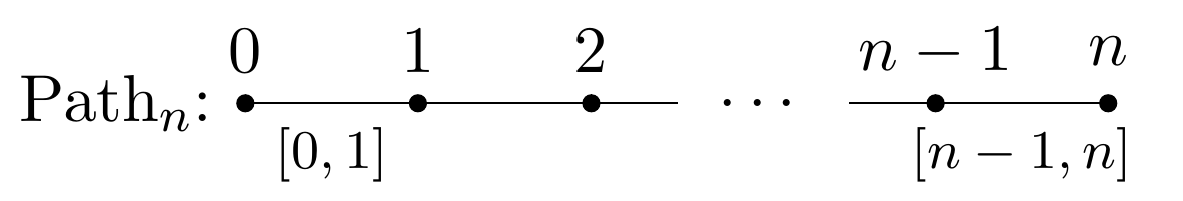
\includegraphics[width=8cm]{assets/path-graph.png}
        \centering
    \end{figure}
    trong đó $\{0,1,...,n\}$ là các đỉnh của đồ thị, $\{[i,i+1] \mid 0 \leq i < n \}$ là các cạnh của đồ thị, với định hướng được xác định bởi $o([i,i+1]) = i$ và $t([i,i+1]) = i+1$.
\end{define}

\begin{define}[\cite{TreeSerre}]
    Một \textdef{đường đi (với chiều dài $n$)} của đồ thị $\Gamma$ là một cấu xạ từ $c: \Path_n \rightarrow \Gamma$.

    Dãy các cạnh $(y_1,...,y_n)$ với $y_i = c([i-1,i])$ sao cho $t(y_i) = o(y_{i+1})$ xác định đường đi $c$. Nếu $P_i = c(i)$ thì ta nói $c$ là đường đi từ $P_0$ đến $P_n$ và ta gọi chung $P_0, P_n$ là các \textdef{đỉnh đầu cuối}.

    Một cặp cạnh có dạng $(y_i,y_{i+1}) = (y_i,\overline{y_i})$ trong đường đi được gọi là \textdef{quay lui}. Bằng cách loại bỏ đi một quay lui, ta có thể xây dựng đường đi mới có độ dài $n-2$ cho bởi $(y_1,...,y_{i-1},y_{y+2},...,y_n)$. Do đó bằng quy nạp, nếu có một đường đi từ $P$ đến $Q$ thì sẽ có một đường đi từ $P$ đến $Q$ không có quay lui.

    Giới hạn trực tiếp $\Path_{\infty} := \varinjlim \Path_n$ cho ta khái niệm về \textdef{đường đi vô hạn}. Nó là một dãy vô hạn các cạnh $(y_1,y_2,...)$ sao cho $t(y_i) = o(y_{i+1})$ với mọi $i \geq 1$.
\end{define}

\begin{define}[\cite{TreeSerre}]
    Một đồ thị được gọi là \textdef{liên thông} nếu luôn có đường đi qua hai đỉnh bất kì trong đồ thị. Đồ thị con liên thông tối đại với quan hệ bao hàm được gọi là \textdef{thành phần liên thông} của đồ thị đó.
\end{define}

\begin{remark}[\cite{TreeSerre}]
    Một đồ thị liên thông khi và chỉ khi nhận dạng của nó liên thông. Hơn nữa, thành phần liên thông của đồ thị tương ứng với thành phần liên thông của nhận dạng.
\end{remark}

\begin{define}[\cite{TreeSerre}]
    Với $n \geq 1$, ta xét đồ thị có hướng
    \begin{figure}[H]
        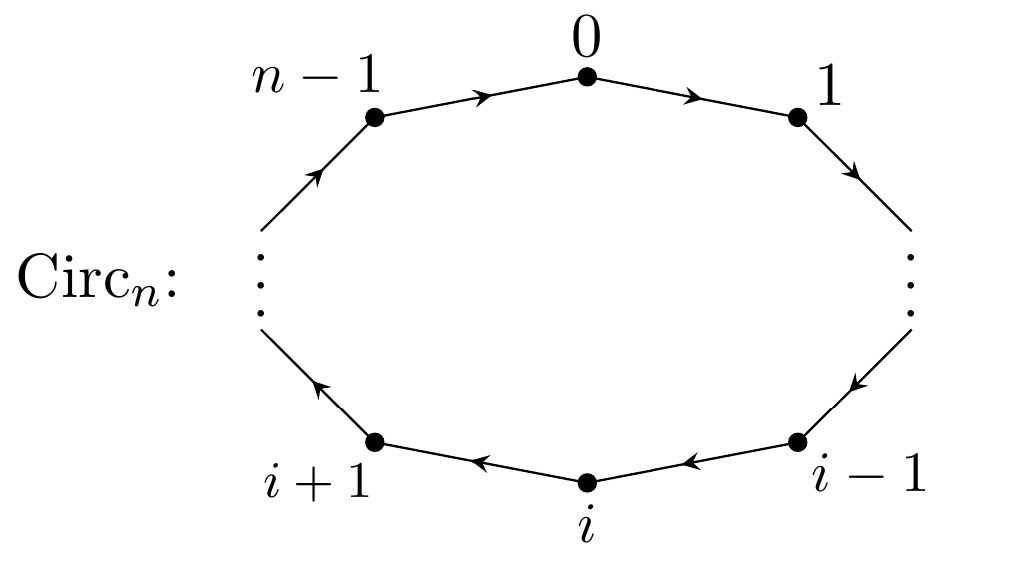
\includegraphics[width=8cm]{assets/circle-graph.png}
        \centering
    \end{figure}
    Trong đó $\Z_n$ là tập các đỉnh, $\{ [i,i+1] \mid i \in \Z_n \}$ là tập các cạnh với định hướng cho bởi $o([i,i+1]) = i$ và $t([i,i+1]) = i + 1$.
\end{define}

\begin{define}[\cite{TreeSerre}]
    Một \textdef{chu trình} độ dài $n$ trong đồ thị bất kì là đồ thị con đẳng cấu với $\Circ_n$.
\end{define}

\begin{define}[\cite{TreeSerre}]
    Một \textdef{cây} là đồ thị liên thông khác rỗng không có chu trình.
\end{define}

% \begin{define}[\cite{TreeSerre}]
%     Cho $G$ là nhóm và $S \subset G$. Ta kí hiệu $\Gamma = \Gamma(G,S)$ là đồ thị có hướng với $G$ là tập đỉnh
% \end{define}
\subsection{Tác động của nhóm lên cây}
\begin{define}[\cite{TreeSerre}]
    Cho $G$ là nhóm và $X$ là đồ thị, một \textdef{tác động} của $G$ lên $X$ là một đồng cấu nhóm $G \rightarrow \Aut(X)$.

    Ta nói $G$ tác động \textdef{tạo cạnh ngược} lên $G$ nếu có phần tử $g \in G$ và cạnh $y \in X$ sao cho $gy = \overline{y}$.

    Nếu $G$ tác động lên $X$ không tạo cạnh ngược thì ta có thể định nghĩa \textdef{đồ thị thương} $G \setminus X$ với tập đỉnh và tập cạnh tương ứng với quỹ đạo dưới tác động $G$ lên $\ver X$ và $\edge X$.

    Nếu $G$ tác động không tạo ra cạnh ngược và không phần tử $g \neq 1$ nào cố định đỉnh của $X$ thì ta nói đây là một \textdef{tác động tự do}.

    Một \textdef{miền cơ bản} của $X$ dưới tác động $G$ là đồ thị con $T$ sao cho cấu xạ cảm sinh $T \rightarrow G \setminus X$ là đẳng cấu. Ta có thể chỉ ra rằng nếu $X$ là cây thì miền cơ bản tồn tại khi và chỉ khi $G \setminus X$ là cây.
\end{define}

\begin{theorem}[\cite{TreeSerre}]\label{thm:bass-serre-fund}
    Cho $G$ là nhóm tác động lên đồ thị $X$, $T$ là cạnh $P \xrightarrow[]{Y} Q$ trong $X$, đồng thời là miền cơ bản của $X$ và kí hiệu $G_P,\ G_Q,\ G_Y$ lần lượt là nhóm con cố định $P$, $Q$ và $Y$. Khi đó $X$ là cây khi và chỉ khi đồng cấu cảm sinh $G_P *_{G_Y} G_Q \rightarrow G$ là đẳng cấu.
\end{theorem}

\subsection{Cây Serre}
Ở phần này ta mặc định $K$ là trường số có định giá rời rạc $v$ và vành định giá $\mathcal{O}$.

\begin{define}[\cite{TreeSerre}]
    Cho $K$ là một trường với vành định giá $\mathcal{O}$. Một \textdef{dàn} trong $K^2$ là một $\mathcal{O}$-môđun tự do có hạng bằng $2$ trong $K^2$.
\end{define}

\begin{remark}[\cite{TreeSerre}]
    Nếu $L$ là dàn trong $K^2$ và $x \in K^*$ thì $L x$ cũng là một dàn, quỹ đạo của $L$ dưới tác động của $K^*$ lên tập các dàn trong $K^2$ được gọi là \textdef{lớp dàn}. Hai dàn $L, L'$ trong $K^2$ được gọi là \textdef{tương đương} nếu chúng cùng nằm trong một lớp dàn, nghĩa là tồn tại phần tử $x \in K^*$ sao cho $L' = L x$, kí hiệu $L \sim L'$.
\end{remark}

\begin{lemma}[\cite{TreeSerre}]
    Nếu $L_0$ và $L_1$ là hai dàn trong $K^2$ thì tồn tại $L_1' \sim L_1$ sao cho $L_1' \subset L_0$.
\end{lemma}

Xét dàn $L_0 = \mathcal{O}v \oplus \mathcal{O}w$ và $L_1$. Từ bổ đề trên, tồn tại $L_1' \sim L_1$ sao cho $L_1' \subset L_0$. Theo Định lí thừa số bất biến của môđun trên vành chính, tồn tại hai số nguyên $a,b$ sao cho
$$
    L_1' = \mathcal{O} \pi^a v \oplus \mathcal{O} \pi^v w,
$$
trong đó $\pi$ là phần tử đồng nhất trong vành định giá $\mathcal{O}$. Khoảng cách giữa hai dàn lúc này được định nghĩa là
$$
    d(L_0, L_1) = |a-b|.
$$
Giá trị $a,b$ ở đây không phụ thuộc vào cách chọn cơ sở cho $\Gamma_0$ và do đó khoảng cách giữa hai dàn được định nghĩa tốt. Hơn nữa nếu ta thay $L_0, L_1$ bởi hai dàn $L_0 x, L_0 y$ $(x,y \in K^*)$ thì hệ số $a,b$ lúc này được thay bằng $a+c, b+c$, trong đó $c = v(y/x)$. Vậy ta có thể nói đến khoảng cách giữa hai lớp dàn tương đương mà không phụ thuộc vào cách chọn phần tử đại diện.

\begin{define_theorem}[\cite{TreeSerre}]
    Đặt $X$ là đồ thị với tập đỉnh là tập các lớp dàn trong $K^2$ và tập cạnh là tập các cặp lớp dàn $(\Lambda,\Lambda')$ sao cho $d(\Lambda,\Lambda') = 1$, ta kí hiệu $\Lambda \Lambda'$ cho một cạnh trong $X$. Lúc này $X$ là cây và $X$ được gọi là \textdef{cây Serre}.
\end{define_theorem}

\startproof Xem \cite[Chương 2, Mục 1.1, Định lí 1]{TreeSerre}.\qed

\subsection{Tác động của $SL_2(K)$ lên cây Serre}

\begin{define}[\cite{TreeSerre}]
    Ta định nghĩa tác động của nhóm $GL_2(K)$ lên dàn $L = \mathcal{O}v \oplus \mathcal{O}w$ cho bởi
    $$
        A(\mathcal{O}v \oplus \mathcal{O}) = \mathcal{O}Av \oplus \mathcal{O}Aw
    $$
    Hơn nữa tác động này bảo toàn khoảng cách giữa hai dàn, do đó $GL_2(K)$ tác động lên cây Serre.
\end{define}

\begin{proposition}[\cite{TreeSerre}]
    Tác động $SL_2(K)$ lên cây Serre giới hạn từ tác động của $GL_2(K)$ không tạo ra cạnh ngược.
\end{proposition}

\begin{theorem}[\cite{TreeSerre}]
    Cho $G$ là nhóm con của $GL_2(K)$. Khi đó nếu bao đóng của $G$ chứa $SL_2(K)$ thì $\Lambda \Lambda'$ là miền cơ bản cho tác động của $G$ lên cây Serre $X$, trong đó $\Lambda \Lambda'$ là một cạnh của $X$. Từ đó dẫn đến
    $$
        G = G_{\Lambda} *_{G_{\Lambda \Lambda'}} G_{\Lambda'},
    $$
    với $G_{\Lambda}, G_{\Lambda'}, G_{\Lambda \Lambda'}$ lần lượt là nhóm con của $G$ cố định $\Lambda, \Lambda'$ và $\Lambda \Lambda'$.
\end{theorem}

\startproof Xem \cite[Chương 2, Mục 1.4, Định lí 2 và Định lí 3]{TreeSerre}.\qed

Bằng cách tính nhóm con cố định đỉnh và cạnh của cây Serre, ta có định lí quan trọng và nổi tiếng sau:

\begin{theorem}[Ihara \cite{TreeSerre}]
    Cho $K$ là trường có định giá rời rạc $v$ với vành định giá $\mathcal{O}$ và phần tử đồng nhất $\pi$. Khi đó
    $$
        SL_2(K) = SL_2(\mathcal{O}) *_\Gamma SL_2(\mathcal{O})
    $$
    % và
    % $$
    %     PSL_2(K) = SL_2(\mathcal{O}) *_{\bar{\Gamma}} PSL_2(\mathcal{O})
    % $$
    với
    $$
        \Gamma = \left\{ \begin{pmatrix}
            * & * \\
            c & *
        \end{pmatrix} \in SL_2(\mathcal{O})\ \middle|\ c \equiv 0\ (\operatorname*{mod}\ \pi) \right\},
    $$
    trong đó hai phép nhúng từ $\Gamma$ vào $SL_2(\mathcal{O})$ cho bởi
    $$
        \begin{pmatrix}
            a & b \\
            c & d
        \end{pmatrix} \mapsto \begin{pmatrix}
            a & b \\
            c & d
        \end{pmatrix}\enskip \text{ và }\enskip \begin{pmatrix}
            a & b \\
            c & d
        \end{pmatrix} \mapsto \begin{pmatrix}
            a         & b\pi         \\
            \pi^{-1}c & \pi^{-1}d\pi
        \end{pmatrix}.
    $$

    % và $\bar{\Gamma} = \Gamma / \{\pm I\}$.
\end{theorem}

\begin{lemma}{\cite{TreeSerre}}
    Nếu $A$ là vành con trù mật trong $K$ thì $SL_2(A)$ trù mật trong $SL_2(K)$.
\end{lemma}
\startproof Bao đóng của $SL_2(A)$ chứa hai nhóm con cộng lần lượt sinh bởi $\begin{pmatrix}
        1 & 1 \\
        0 & 1
    \end{pmatrix}$ và $\begin{pmatrix}
        1 & 0 \\
        1 & 1
    \end{pmatrix}$. Hơn nữa hai ma trận này sinh ra $SL_2(K)$.\qed

\begin{corollary}[\cite{TreeSerre}]\label{cor:amalgam-sl2-1p}
    Với $p$ là số nguyên tố, ta có
    $$
        SL_2(\Z[1/p]) \cong SL_2(\Z) *_{\Gamma_0(p)} SL_2(\Z),
    $$
    trong đó $\Gamma_0(p)$ là nhóm con đồng dư Hecke của $SL_2(\Z)$.
\end{corollary}

\startproof Xem \cite[Chương 2, Mục 1.4, Hệ quả 2]{TreeSerre}.\qed

Từ đó ta có một kết quả tổng quát như sau:

\begin{corollary}[\cite{TreeSerre}]\label{cor:sl2-amalgam}
    Nếu $n$ là số nguyên không có ước nguyên tố $p$ thì khi đó
    $$
        SL_2(\Z[1/pn]) \cong SL_2(\Z[1/n]) *_{\Gamma} SL_2(\Z[1/n]).
    $$
    trong đó
    $$
        \Gamma = \left\{ \begin{pmatrix}
            * & * \\
            c & *
        \end{pmatrix} \in SL_2(\Z[1/n])\ \middle|\ c \equiv 0\ (\operatorname*{mod}\ \pi) \right\}.
    $$
    Vậy nhóm $SL_2(\Z[1/p_1...p_k])$ có thể biểu diễn thành tích amalgam của các nhóm $SL_2(\Z)$ trên các nhóm con đồng dư. Đây là kết quả quan trọng trong công cuộc tính đối đồng điều của nhóm $SL_2(\Z[1/m])$ với $m$ là tích các số nguyên tố phân biệt bất kì.
\end{corollary}
\section{Đại số đồng điều}

Trong mục này, nếu không giải thích gì thêm, ta mặc định coi $R$ là vành giao hoán có đơn vị và khi nhắc đến một môđun thì ta hiểu đó là một $R$-môđun trái.
\begin{define}
    Một \textdef{phức dây chuyền} là một cặp $(C,d)$,  trong đó $C = \{ C_n \}_{n \in \Z}$ là một họ các môđun và $d = \{d_n: C_n \rightarrow C_{n-1}\}_{n \in \Z}$ là một họ các đồng cấu thỏa mãn $d_n \circ d_{n+1} = 0$.

    $$
        \begin{tikzcd}
            \cdots \arrow[r] & C_2 \arrow[r, "d_2"] & C_1 \arrow[r, "d_1"] & C_0 \arrow[r, "d_0"] & C_{-1} \arrow[r] & \cdots
        \end{tikzcd}
    $$
    Một \textdef{phức đối dây chuyền} là một cặp $(C,d)$,  trong đó $C = \{ C_n \}_{n \in \Z}$ là một họ các môđun và $d = \{d^n: C^n \rightarrow C^{n+1}\}_{n \in \Z}$ là một họ các đồng cấu thỏa mãn $d^n \circ d^{n-1} = 0$.

    $$
        \begin{tikzcd}
            \cdots & C^2 \arrow[l] & C^1 \arrow[l, "d^1"'] & C^0 \arrow[l, "d^0"'] & C^{-1} \arrow[l, "d^{-1}"'] & \cdots \arrow[l]
        \end{tikzcd}
    $$
    Ngoài ra để ngắn gọn, ta có thể gọi \textdef{phức} hay \textdef{đối phức} thay cho phức dây chuyền và đối phức dây chuyền.
\end{define}

Từ đó ta định nghĩa \textdef{đồng điều} của một phức $(C,d)$ là họ các nhóm Abel
$$
    H_n(C) = \ker d_n / \im d_{n+1}
$$
và \textdef{đối đồng điều} của một đối phức $(C,d)$ là họ các nhóm Abel
$$
    H^n(C) = \ker d^n / \im d^{n-1},
$$
trong đó ta gọi
\begin{itemize}
    \item $c \in \ker d_n$ là một \textdef{chu trình $n$ chiều}.
    \item $c \in \ker d^n$ là một \textdef{đối chu trình $n$ chiều}.
    \item $b \in \im d_{n+1}$ là một \textdef{biên $n$ chiều}.
    \item $b \in \im d_{n+1}$ là một \textdef{đối biên $n$ chiều}.
\end{itemize}
Hơn nữa ta kí hiệu $[c]$ cho ảnh của $c$ trong $H_n(C)$ nếu $c$ là chu trình và là ảnh của $c$ trong $H^n(C)$ nếu $c$ là đối chu trình.

\begin{define}
    Cho $(C,d)$ và $(D,d')$ là các phức (tương ứng đối phức). Một \textdef{ánh xạ dây chuyền} $f: C \rightarrow D$ là một họ các đồng cấu $f_n: C_n \rightarrow D_n$ (tương ứng $f^n: C^n \rightarrow D^n$), $n \in \Z$, sao cho biểu đồ sau giao hoán
    \begin{eqnarray*}
        \begin{tikzcd}
            C_n \arrow[d, "f_n"'] \arrow[r, "d_n"] & C_{n-1} \arrow[d, "f_{n-1}"] \\
            D_n \arrow[r, "d'_n"']                 & D_{n-1}
        \end{tikzcd}
        &
        \left(\text{tương ứng}\quad \begin{tikzcd}
            C^n \arrow[r, "d^n"] \arrow[d, "f_n"'] & C^{n+1} \arrow[d, "f_{n+1}"] \\
            D^n \arrow[r, "d'^n"']                 & D^{n+1}
        \end{tikzcd}\right).
    \end{eqnarray*}

    Một \textdef{đồng luân} $h$ giữa hai ánh xạ dây chuyền $f,g: (C,d) \rightarrow (D,d')$ là họ các đồng cấu $h_n: C_n \rightarrow D_{n+1}$ sao cho $d'_{n+1} \circ h_n + h_{n-1} \circ d_n = f_n - g_n$. Đồng luân thường được minh họa thông qua biểu đồ sau, tuy nhiên đây không phải là biểu đồ giao hoán.
    % https://q.uiver.app/#q=WzAsMTAsWzIsMCwiQ19uIl0sWzMsMCwiQ197bi0xfSJdLFsxLDAsIkNfe24rMX0iXSxbMSwxLCJEX3tuKzF9Il0sWzIsMSwiRF9uIl0sWzMsMSwiRF97bi0xfSJdLFswLDAsIlxcY2RvdHMiXSxbMCwxLCJcXGNkb3RzIl0sWzQsMCwiXFxjZG90cyJdLFs0LDEsIlxcY2RvdHMiXSxbMiwzLCIiLDAseyJvZmZzZXQiOjF9XSxbMiwzLCIiLDIseyJvZmZzZXQiOi0xfV0sWzAsNCwiZl9uIiwyLHsib2Zmc2V0IjoxLCJjb2xvdXIiOlszNTksMTAwLDYwXX0sWzM1OSwxMDAsNjAsMV1dLFswLDQsImdfbiIsMCx7Im9mZnNldCI6LTEsImNvbG91ciI6WzM1OSwxMDAsNjBdfSxbMzU5LDEwMCw2MCwxXV0sWzEsNSwiIiwwLHsib2Zmc2V0IjoxfV0sWzEsNSwiIiwyLHsib2Zmc2V0IjotMX1dLFsyLDBdLFszLDQsImQnX3tuKzF9IiwyLHsiY29sb3VyIjpbMzU5LDEwMCw2MF19LFszNTksMTAwLDYwLDFdXSxbNCw1XSxbMCwzLCJoX24iLDEseyJjb2xvdXIiOlszNTksMTAwLDYwXX0sWzM1OSwxMDAsNjAsMV1dLFsxLDQsImhfe24tMX0iLDEseyJjb2xvdXIiOlszNTksMTAwLDYwXX0sWzM1OSwxMDAsNjAsMV1dLFswLDEsImRfbiIsMCx7ImNvbG91ciI6WzM1OSwxMDAsNjBdfSxbMzU5LDEwMCw2MCwxXV0sWzYsMl0sWzcsM10sWzEsOF0sWzUsOV1d
    \[\begin{tikzcd}
            \cdots & {C_{n+1}} & {C_n} & {C_{n-1}} & \cdots \\
            \cdots & {D_{n+1}} & {D_n} & {D_{n-1}} & \cdots
            \arrow[from=1-1, to=1-2]
            \arrow[from=1-2, to=1-3]
            \arrow[shift right, from=1-2, to=2-2]
            \arrow[shift left, from=1-2, to=2-2]
            \arrow["{d_n}", color={mycolor}, from=1-3, to=1-4]
            \arrow["{h_n}"{description}, color={mycolor}, from=1-3, to=2-2]
            \arrow["{f_n}"', shift right, color={mycolor}, from=1-3, to=2-3]
            \arrow["{g_n}", shift left, color={mycolor}, from=1-3, to=2-3]
            \arrow[from=1-4, to=1-5]
            \arrow["{h_{n-1}}"{description}, color={mycolor}, from=1-4, to=2-3]
            \arrow[shift right, from=1-4, to=2-4]
            \arrow[shift left, from=1-4, to=2-4]
            \arrow[from=2-1, to=2-2]
            \arrow["{d'_{n+1}}"', color={mycolor}, from=2-2, to=2-3]
            \arrow[from=2-3, to=2-4]
            \arrow[from=2-4, to=2-5]
        \end{tikzcd}\]

    Nếu tồn tại một đồng luân như vậy thì ta nói $f$ đồng luân với $g$. Kí hiệu $f \simeq g$.
\end{define}

\begin{lemma}\label{lem:extend_chain_map}
    Cho $(C,d)$ và $(D,d')$ là các phức, $k \in \Z$ và $\{f_i: C_i \rightarrow D_i\}_{i \leq k}$ là họ các đồng cấu thỏa $d_i' \circ f_i = f_{i-1} \circ d_i$ với $i \leq k$. Nếu $C_i$ là môđun xạ ảnh với mọi $i > k$ và $H_i(D) = 0$ với mọi $i \geq k$ thì khi đó $\{f_i\}_{i \leq k}$ mở rộng thành ánh xạ dây chuyền $f: C \rightarrow D$. Hơn nữa $f$ xác định duy nhất sai khác một đồng luân.
\end{lemma}

\begin{define}
    Một \textdef{phép giải} của môđun $M$ trên $R$ là một dãy khớp các $R$-môđun
    $$
        \begin{tikzcd}
            \cdots \arrow[r] & P_2 \arrow[r, "d_2"] & P_1 \arrow[r, "d_1"] & P_0 \arrow[r, "\varepsilon"] & M \arrow[r] & 0
        \end{tikzcd}
    $$
    % Ta kí hiệu phép giải trên bằng bộ $(P,d,\epsilon)$.

    Nếu $\{P_n\}$ là các môđun tự do (tương ứng môđun xạ ảnh) thì phép giải trên được gọi là \textdef{phép giải tự do} (tương ứng \textdef{phép giải xạ ảnh}).

    Nếu tồn tại chỉ số $n \in \N$ nào đó để $P_n \neq 0$ và $P_{k} = 0$ với mọi $k \geq n$ thì khi đó ta nói phép giải trên hữu hạn với độ dài $n$.
\end{define}

\begin{define}
    Cho $M,A$ là các môđun và $(P,d,\varepsilon)$ là một phép giải xạ ảnh của $M$. Khi đó ta định nghĩa $\Tor_n^R(M,A)$ là đồng điều bậc $n$ của phức dây chuyền
    $$
        \begin{tikzcd}
            \cdots \arrow[r] & P_2 \otimes A \arrow[r, "d_2 \otimes 1"] & P_1 \otimes A \arrow[r, "d_1 \otimes 1"] & P_0 \otimes A \arrow[r] & 0
        \end{tikzcd}
    $$
    và $\Ext^n_R(M,A)$ là đồng điều bậc $n$ của phức dây chuyền
    $$
        \begin{tikzcd}
            \cdots \arrow[r] & {\Hom(P_2,A)} & {\Hom(P_1,A)} \arrow[l, "\delta^1"'] & {\Hom(P_0,A)} \arrow[l, "\delta^0"'] & 0 \arrow[l]
        \end{tikzcd}
    $$
    trong đó $\delta^n = \square \circ d_{n+1}$.

    Hai định nghĩa trên đều được định nghĩa tốt, nghĩa là $\Tor_n^R(M,A)$ và $\Ext^n_R(M,A)$ không phụ thuộc vào phép giải xạ ảnh của $M$. Trong trường hợp vành $R$ không gây sự nhầm lẫn thì ta có thể lược bỏ chỉ số $R$ của $\Tor$ và $\Ext$ cho ngắn gọn. Hơn nữa ta kí hiệu $\Tor(M,A)$ thay cho $\Tor_1(M,A)$ và $\Ext(M,A)$ thay cho $\Ext^1(M,A)$.
\end{define}

\begin{proposition}[\cite{HatcherAT}]\label{prop:ext-props}
    Nhóm $\Ext$ trong một vài trường hợp cụ thể có thể dễ dàng tính toán được dựa trên một số tính chất sau:
    \begin{itemize}
        \item $\Ext^n(M_1 \oplus M_2, A) \cong \Ext^n(M_1,A) \oplus \Ext^n(M_2,A)$.
        \item $\Ext(M, A) = 0$ nếu $M$ xạ ảnh.
        \item $\Ext(\Z/m, G) \cong G/mG$, trong đó $G$ là nhóm Abel.
    \end{itemize}
\end{proposition}

\begin{theorem}[Định lí hệ số phổ dụng cho đối đồng điều]
    Cho $R$ là vành giao hoán, $M$ là $R$-môđun và $C$ là phức các $R$-môđun. Khi đó ta có dãy khớp chẻ
    $$
        0 \rightarrow \Ext_R(H_{n-1}(C), M) \rightarrow H^n(C;M) \rightarrow \Hom_R(H_n(C), M) \rightarrow 0.
    $$
\end{theorem}

\startproof Xem \cite[Định lí 3.2]{HatcherAT}.\qed

Định lí này là một công cụ mạnh mẽ giúp ta tính đối đồng điều của nhóm. Cụ thể trong trường hợp $M = R = \Z$, ta có hệ quả sau.

\begin{corollary}\label{cor:universal-coef}
    Cho $C$ là phức các nhóm Abel, $n \in \N$ và giả sử $H_n(C;\Z)$ hữu hạn sinh, tức là ta có phân tích
    $$
        H_n(C;\Z) \cong \Z^{b_n} \oplus T_n,
    $$
    với $T_n$ là nhóm xoắn. Khi đó
    $$
        H^n(C;\Z) \cong \Z^{b_n} \oplus T_{n-1}.
    $$
\end{corollary}

\startproof Ta có
$$
    \Hom(H_n(C), \Z) \cong \Hom(\Z^{b_n}, \Z) \oplus \Hom(T_n, \Z) \cong \Z^{b_n}
$$
và từ Mệnh đề \ref{prop:ext-props} ta suy ra được
$$
    \Ext(H_{n-1}(C), \Z) \cong \Ext(\Z^{b_{n-1}}, \Z) \oplus \Ext(T_{n-1}, \Z) \cong T_{n-1}.
$$
Áp dụng Định lí hệ số phổ dụng cho đối đồng điều, ta có điều phải chứng minh. \qed
\section{(Đối) đồng điều nhóm}

\begin{define}[\cite{ClaraGroupCohom}]
    Cho $G$ là nhóm và $R$ là vành giao hoán. Ta định nghĩa \textdef{vành nhóm} $RG$ là $R$-môđun tự do sinh bởi các phần tử trong $G$. Do đó mỗi phần tử trong $RG$ có biểu diễn duy nhất dưới dạng tổng hữu hạn $\sum_{g \in G} a_g g$, trong đó $a_g \in R,\ g \in G$. Hơn nữa $RG$ có cấu trúc vành cho bởi phép nhân
    $$
        \left(\sum_{g\in G}a_g g\right)\left(\sum_{g\in G}b_g g\right) = \sum_{g\in G} \left(\sum_{h \in G}a_h b_{h^{-1}g}\right) g.
    $$
\end{define}

\begin{define}
    Nếu nhóm $G$ tác động lên tập $M$ thì ta có thể coi $M$ là một $\Z G$-môđun, hay ngắn gọn hơn, ta gọi $M$ là một \textdef{$G$-môđun}.
\end{define}

\begin{define}
    Một $G$-môđun $M$ được gọi là \textdef{tầm thường} nếu $gm = m$ với mọi $g \in G$ và $m \in M$.
\end{define}

Nếu không giải thích gì thêm thì ta mặc định cấu trúc $G$-môđun của $\Z$ là tầm thường.

\begin{define}
    Cho $G$ là nhóm và $M$ là một $G$-môđun. Ta định nghĩa
    $$
        H_n(G;M) = \Tor_n^{\Z G}(\Z,M)
    $$
    là \textdef{đồng điều thứ $n$ của nhóm $G$ với hệ số $M$}. Tương tự ta định nghĩa
    $$
        H^n(G;M) = \Ext^n_{\Z G}(\Z,M).
    $$
    là \textdef{đối đồng điều thứ $n$ của nhóm $G$ với hệ số $M$}. Trong trường hợp hệ số $M = \Z$ thì ta gọi đơn giản $H_n(G;\Z)$ và $H^n(G;\Z)$ là đồng điều và đối đồng điều thứ $n$ của nhóm $G$.
\end{define}

\begin{define}[\cite{ClaraGroupCohom}]
    Cho $G$ là nhóm và $M$ là một $G$-môđun. Ta định nghĩa
    $$
        M^G = \{ m \in M\ |\ gm = m \}
    $$
    là \textdef{nhóm các bất biến} của $M$ và
    $$
        M_G = M / \langle g m - m\ |\ g \in G, m \in M \rangle_\Z
    $$
    là \textdef{nhóm các đối bất biến} của $M$. Có thể hiểu $M^G$ là nhóm con lớn nhất của $M$ mà $G$ tác động tầm thường lên, trong khi đó $M_G$ là nhóm thương lớn nhất của $M$ để  $G$ tác động tầm thường. Ta có thể kiểm tra được
    \begin{align*}
        \cdot_G: {}_{\Z G}\textbf{Mod} \rightarrow {}_{\Z}\textbf{Mod} \\
        \cdot^G: {}_{\Z G}\textbf{Mod} \rightarrow {}_{\Z}\textbf{Mod}
    \end{align*}
    lần lượt là hàm tử và phản hàm tử.
\end{define}

\begin{proposition}[\cite{ClaraGroupCohom}]
    Cho $G$ là nhóm và $M$ là một $G$-môđun. Khi đó
    \begin{align*}
        M_G & \longrightarrow M \otimes_G \Z \\
        [a] & \longmapsto a \otimes 1
    \end{align*}
    và
    \begin{align*}
        M^G & \longrightarrow \Hom_G(\Z,M)      \\
        a   & \longmapsto (n \mapsto n \cdot a)
    \end{align*}
    là các đẳng cấu nhóm. Điều này cũng có nghĩa là $H_0(G;M) \cong M_G$ và $H^0(G;M) \cong M^G$.
\end{proposition}

\begin{theorem}[\cite{ClaraGroupCohom}]\label{thm:first-homology}
    Cho $G$ là nhóm. Khi đó
    $$
        H_1(G;\Z) \cong G^{\ab} = G/[G,G].
    $$
\end{theorem}
\startproof Xem \cite[Định lí 1.4.1]{ClaraGroupCohom}.

\begin{proposition}\label{prop:cohom-coef-prod}
    Cho tích $M = \prod_i M_i$ các $G$-môđun, khi đó bản thân $M$ có cấu trúc $G$-môđun thông qua tác động đường chéo
    $$
        g(m_1,m_2,...) = (gm_1, gm_2,...).
    $$
    Hơn nữa
    $$
        H^k(G; M) \cong \prod_i H^r(G; M_i).
    $$
\end{proposition}

\subsection{(Đối) đồng điều nhóm với góc nhìn tôpô}
Ở phần này ta sẽ thấy rằng bằng cách coi $G$ như một không gian tôpô thông qua không gian phân loại thì (đối) đồng điều mà ta định nghĩa trên nhóm cũng chính là (đối) đồng điều trên tôpô theo nghĩa cổ điển.

\begin{proposition}\label{prop:free-G-action}
    Cho nhóm $G$ tác động tự do lên $X$ và $E$ là tập các phần tử đại diện của các $G$-quỹ đạo trong $X$. Khi đó $X$ là một $\Z G$-môđun tự do với cơ sở $E$.
\end{proposition}
\startproof
Ta biết rằng $G(x)$ và $G/G_x$ có cùng lực lượng, hơn nữa $G/G_x \cong G$ do $G$ tác động tự do lên $X$, do đó
$$
    \Z[X] = \Z\left[\bigsqcup_{x \in E} G(x)\right] = \bigoplus_{x \in E} \Z[G(x)] \cong \bigoplus_{x \in E} \Z[G/G_x] \cong \bigoplus_{x \in E} \Z G.
    \eqno\qed
$$
\begin{define}[\cite{CohomBrown}]
    Cho $G$ là nhóm, ta nói $X$ là một \textdef{$G$-phức} nếu $X$ là CW-phức với tác động $G$ lên các ô của $X$. Từ đó $G$ cũng cảm sinh ra một tác động lên $X$. Nếu tác động này là tác động tự do thì ta nói $X$ là một \textdef{$G$-phức tự do}.
\end{define}

Nếu $X$ là $G$-phức thì tác động của $G$ lên các ô của $X$ mở rộng thành tác động lên $C_n(X)$, khi đó $C(X)$ trở thành phức dây chuyền của các $G$-môđun. Hơn nữa \textdef{ánh xạ tăng cường} (augmentation map) $\varepsilon: C_0(X) \rightarrow \Z$ cho bởi $\varepsilon(v) = 1$ là đồng cấu $G$-môđun thỏa $\varepsilon \circ d = 0$. Khi đó $C_*(X) \xrightarrow{\varepsilon} \Z$ là một dãy phức các $G$-môđun, ta gọi là \textdef{dãy phức ô tăng cường} (augmented
cellular chain complex).

\begin{proposition}[\cite{CohomBrown}]\label{prop:free-cell-resolution}
    Cho $X$ là $G$-phức tự do co rút được. Khi đó dãy phức ô tăng cường trên là một phép giải tự do.
\end{proposition}
\startproof Từ Mệnh đề \ref{prop:free-G-action} ta có $C_*(X)$ là các $G$-môđun tự do, tính khớp được suy ra từ việc tất cả các đồng điều của $C_*(X)$ bằng $0$.\qed

\begin{remark}
    Giả sử $Y$ là CW-phức và $p: \tilde{Y} \rightarrow Y$ là một ánh xạ phủ chính quy với $G$ là nhóm các biến đổi phủ (deck transformation). Khi đó $\tilde{Y}$ là một $G$-phức tự do và $C_*(\tilde{Y})$ là $G$-môđun tự do có cơ sở là các ô trong $Y$.
    % TOPROOF
\end{remark}

\begin{define}[\cite{CohomBrown}]
    Với góc nhìn ở nhận xét trên và Mệnh đề \ref{prop:free-cell-resolution} thì ta mong muốn sự tồn tại của một CW-phức $Y$ thỏa các tính chất:
    \begin{enumerate}[(i)]
        \item $Y$ liên thông.
        \item $\pi_1(Y) = G$.
        \item Phủ phổ dụng của $Y$ co rút được.
    \end{enumerate}
    Một phức $Y$ như vậy được gọi là \textbf{không gian phân loại của} $G$ hay \textbf{phức Eilenberg-Maclane loại} $(G,1)$, hay đơn giản hơn là $K(G,1)$-phức. Cuối cùng từ các ý tưởng trên ta có mệnh đề sau.
\end{define}

\begin{proposition}[\cite{CohomBrown}]
    Nếu $Y$ là không gian phân loại của $G$ với phủ phổ dụng $X$. Khi đó dãy phức ô tăng cường $C_*(X) \rightarrow \Z$ là một phép giải tự do của $\Z$ trên $\Z G$.
\end{proposition}

Hơn nữa ta có thể chỉ ra được sự tồn tại của không gian phân loại của $G$.
% \begin{define}
%     Một \textdef{đơn hình chuẩn $n$ chiều} $\Delta_n$ được định nghĩa là bao đóng lồi của $n+1$ điểm $(1,0,...,0), (0,1,...,0),...,(0,0,...,1) \in \R^{n+1}$ với tôpô cảm sinh từ tôpô Euclid trên $\R^{n+1}$. Bao đóng lồi của một tập con bất kì của $n+1$ điểm trên được gọi là \textdef{mặt} của $\Delta_n$.

%     Một cấu trúc \textdef{$\Delta$-phức} của không gian tôpô $X$ là một họ các ánh xạ liên tục $K = \{\sigma_\alpha: \Delta_{n_\alpha} \rightarrow X\}_{\alpha \in I}$ thỏa:
%     \begin{itemize}
%         \item $\sigma_{\alpha}$ giới hạn trên $\interior(\Delta_{n_\alpha})$ là đơn ánh và ảnh của chúng rời nhau đôi một.
%         \item Giới hạn của $\sigma_\alpha$ lên mặt bất kì của $\Delta_{n_\alpha}$ là một $\sigma_\beta: \Delta_{n_\alpha -  1} \rightarrow X$ nào đó.
%         \item $A \subset X$ mở khi và chỉ khi $\sigma_\alpha^{-1}(A)$ mở trong $\Delta_{n_\alpha}$ với mọi $\alpha$.
%     \end{itemize}
%     Ảnh của $\sigma_\alpha$ được gọi là một \textdef{đơn hình $n_\alpha$ chiều}.
% \end{define}

\begin{proposition}
    Mọi nhóm đều có không gian phân loại.
\end{proposition}
\startproof Cho $G$ là một nhóm. Ta sẽ đi xây dựng phức đơn hình $EG$ như sau: mỗi bộ $n+1$ phần tử $[g_0,...,g_n]$ trong $G$ là một phức đơn hình $n$ chiều của $EG$. $EG$ co rút được thông qua phép đồng luân $h_t$ đẩy một phần tử $x \in [g_0,...,g_n]$ đến điểm $[e]$ theo đoạn thẳng trong $[e,g_0,...,g_n]$.

$G$ tác động lên $EG$ thông qua phép nhân trái
$$
    g \cdot [g_0,...,g_n] = [gg_0,...,gg_n].
$$
Hơn nữa ta có thể kiểm tra được tác động này là một tác động phủ. Do đó ánh xạ thương $EG \rightarrow EG / G$ là một phủ phổ dụng của không gian quỹ đạo $BG = EG/G$. Vậy $BG$ chính là một không gian phân loại của $G$.\qed
% \startproof Cho $G$ là một nhóm và đặt $EG$ là $\Delta$-phức với đơn hình $n$ chiều trong $EG$ có dạng một bộ $n+1$ phần tử $[g_0,...,g_n]$ trong $G$.

\begin{proposition}
    Nếu $Y$ là không gian phân loại của $G$. Khi đó $H_*(Y) \cong H_*(G)$ và $H^*(Y;M) \cong H^*(G;M)$ với mọi $G$-môđun $M$.
\end{proposition}

% \begin{define}
%     Cho đồng cấu nhóm $\alpha: G \rightarrow G'$ với $C$ và $D$ lần lượt là phép giải của $\Z$ trên $\Z G$ và $\Z G'$. Ta có thể coi $D$ là $G$-môđun thông qua $\alpha$. Từ Bổ đề \ref{lem:extend_chain_map}, ta có thể xây dựng
% \end{define}

\subsection{(Đối) đồng điều của nhóm cyclic}
Đây là một ví dụ đơn giản cho việc tính toán đối đồng điều của nhóm, đồng thời cũng là một kết quả cần thiết để ta tính đối đồng điều của $SL_2(\Z)$ ở phần sau.

Cho $G$ là nhóm cyclic cấp $n$ với $t$ là phần tử sinh. Xét $N = \sum_{i=0}^{n-1} t^i$ và $t-1$ là các phần tử trong $\Z G$. Để ý rằng $(t-1) N = t^n - 1 = 0$, hơn nữa $N$ và $t-1$ đều là các phần tử bất khả quy trên $\Z G$. Do đó $\langle N\rangle = \ker(t-1)$ và $\langle t-1 \rangle = \ker(N)$. Từ đó ta có phép giải tự do sau
$$
    \begin{tikzcd}
        \cdots \arrow[r, "t-1"] & \Z G \arrow[r, "N"] & \Z G \arrow[r, "t-1"] & \Z G \arrow[r, "\epsilon"] & \Z \arrow[r] & 0
    \end{tikzcd}
$$
Tác động hàm tử $\Hom_{\Z G}(-,\Z)$ ta được dãy phức
$$
    \begin{tikzcd}
        \Hom_{\Z G}(\Z G,\Z) \arrow[r, "t-1"] & \Hom_{\Z G}(\Z G,\Z) \arrow[r, "N"] & \Hom_{\Z G}(\Z G,\Z) \arrow[r, "t-1"] & \cdots
    \end{tikzcd}
$$
với $N$ và $t-1$ được xác định thông qua tác động lên $f \in \Hom_{\Z G}(\Z G, \Z)$. Nhưng do $G$ tác động tầm thường lên $\Z$ nên tác động bởi $t-1$ tương ứng với đồng cấu không và tác động bởi $N$ tương ứng với đồng cấu cộng $n$ lần. Do đó dãy phức trên tương đương với
$$
    \begin{tikzcd}
        \Z \arrow[r, "0"] & \Z \arrow[r, "n"] & \Z \arrow[r, "0"] & \Z \arrow[r, "n"] & \cdots
    \end{tikzcd}
$$
Suy ra đối đồng điều thứ $k$ của $G$ là
$$
    H^k(G;\Z) = \begin{cases}
        \Z,   & k = 0              \\
        0,    & k \text{ lẻ}       \\
        \Z/n, & k > 0 \text{ chẵn}
    \end{cases}
$$
Từ hệ quả của Định lí hệ số phổ dụng \ref{cor:universal-coef}, ta có
$$
    H_k(G;\Z) = \begin{cases}
        \Z,   & k = 0              \\
        \Z/n, & k \text{ lẻ}       \\
        0,    & k > 0 \text{ chẵn}
    \end{cases}
$$

% \subsection{Môđun cảm sinh và đối cảm sinh}
% \begin{define}
%     Cho $G$ là nhóm, $H \leq G$ và $M$ là $H$-môđun. Ta gọi mở rộng vành hệ tử của $M$ cảm sinh từ đơn cấu vành $\Z G \hookrightarrow \Z H$ là \textdef{môđun cảm sinh} từ $H$ vào $G$, kí hiệu
%     $$
%         \Ind^G_H M = \Z G \otimes_{\Z H} M.
%     $$
%     Tương tự ta định nghĩa \textdef{môđun đối cảm sinh} từ $H$ vào $G$
%     $$
%         \Coind^G_H M = \Hom_{\Z H}(\Z G, M).
%     $$
% \end{define}

% \begin{define}
%     Cho $G$ là nhóm hữu hạn và $M$ là một $ G$-môđun. Với $n > 0$, đặt
%     $$
%         C^n(G,M) = \{ f: G^n \rightarrow M \}
%     $$
%     là tập các \textdef{đối dây chuyền $n$ chiều}. Quy ước $C^0(G,M) = M$ và $C^n(G,M) = 0$ với $n < 0$. Từ đó ta định nghĩa toán tử đối biên $\delta^n: C^n(G,M) \rightarrow C^{n+1}(G,M)$ xác định bởi
%     \begin{align*}
%         (\delta^n f)(g_1,...,g_n) = & g_0f(g_1,...,g_n)                                                 \\
%         +                           & \sum_{j=1}^n (-1)^j f(g_0,...,g_{j-2},g_{j-1}g_j,g_{j+1},...,g_n) \\
%         +                           & (-1)^{n+1} f(g_0,...,g_{n-1})
%     \end{align*}
%     với $n > 1$.
% \end{define}
\subsection{(Đối) đồng điều của tích amalgam}
Trong phần này ta sẽ đưa ra dãy khớp dài để tính (đối) đồng điều của tích amalgam từ các nhóm cấu thành. Trước tiên ta nhắc lại Định lí Seifert–Van Kampen theorem ở dạng CW-phức.

\begin{theorem}
    Cho $X$ là CW-phức, trong đó $X = X_1 \cup X_2$ có phần giao $Y = X_1 \cap X_2$ liên thông khác rỗng. Khi đó ta có phân tích
    $$
        \pi_1 X = \pi_1 X_1 *_{\pi_1 Y} \pi_1 X_2.
    $$
    Nói theo ngôn ngữ phạm trù thì $\pi_1: \textbf{Complex} \rightarrow \textbf{Grp}$ là hàm tử bảo toàn tích amalgam. Để nghiên cứu đối đồng điều nhóm, ta mong muốn hàm tử $K(-,1)$ đi chiều ngược lại và cũng bảo toàn tích amalgam. Thật vậy, miễn là hai ánh xạ $f_1, f_2$ trong phân tích là đơn ánh thì điều này hoàn toàn đúng.
\end{theorem}

\begin{theorem}[\cite{CohomBrown}]
    Mọi phân tích amalgam $G_1 *_A G_2$ trên nhóm
    $$
        \begin{tikzcd}
            A \arrow[d, "f_2"'] \arrow[r, "f_1"] & G_1 \arrow[d] \\
            G_2 \arrow[r]                        & G
        \end{tikzcd}
    $$
    với $f_1, f_2$ là đơn ánh đều nhận được từ nhóm cơ bản của các không gian phân loại
    $$
        \begin{tikzcd}
            Y \arrow[r, hook] \arrow[d, hook] & X_1 \arrow[d, hook] \\
            X_2 \arrow[r, hook]               & X
        \end{tikzcd}
    $$
    trong đó $Y,X_1,X_2,X$ lần lượt là không gian phân loại của $A,G_1,G_2,G$.
\end{theorem}

\begin{proposition}[\cite{CohomBrown}]\label{prop:long-seq-amalgam}
    Cho $G = G_1 *_A G_2$ với các đồng cấu nhúng $\alpha_1: A \rightarrow G_1$ và $\alpha_2: A \rightarrow G_2$. Khi đó ta có dãy khớp dài các đồng điều nhóm
    $$
        \cdots \xrightarrow{} H_n(A) \xrightarrow{} H_n(G_1) \oplus H_n(G_2) \xrightarrow{} H_n(G) \xrightarrow{} H_{n-1}(A) \xrightarrow{} \cdots
    $$
    và dãy khớp dài các đối đồng điều nhóm với hệ số trong $G$-môđun $M$
    $$
        \cdots \xrightarrow{} H^n(A;M) \xrightarrow{} H^n(G_1;M) \oplus H^n(G_2;M) \xrightarrow{} H^n(G;M) \xrightarrow{} H^{n-1}(A;M) \xrightarrow{} \cdots
    $$
\end{proposition}

\section{Dãy phổ}

\subsection{Dãy phổ của phức lọc}
Nếu $C$ là phức và $C'$ là phức con của $C$, khi đó ta biết rằng có một dãy khớp dài cho ta thông tin của $H_*(C)$ dựa trên các hạng tử $H_*(C')$ và $H_*(C/C')$. Bây giờ trong trường hợp thay vì ta có phức con $C'$ đơn lẻ thì ta có một dãy lọc các phức con $\{F_pC\}_{p \in \Z}$ thỏa $F_{p-1}C \subset F_pC$. Lúc này ta cũng muốn có một công cụ để chắt lọc thông tin của $H_*(C)$ từ $H_*(F_pC / F_{p-1}C)$.

\begin{define}[\cite{CohomBrown}]
    Cho $R$ là vành và $M$ là $R$-môđun. Một \textdef{lọc tăng} của $M$ là một dãy các $R$-môđun con $F_pM (p \in \Z)$ thỏa $F_pM \subset F_{p+1}M$. Lọc này được gọi là hữu hạn nếu $F_pM = 0$ với $p$ đủ nhỏ và $F_pM = M$ với $p$ đủ lớn. Hơn nữa ta định nghĩa \textdef{môđun phân bậc} $\Gr M$ tương ứng với một lọc cho bởi $\Gr_p M = F_pM / F_{p-1}M$.

    Trong trường hợp bản thân $M$ là môđun phân bậc, với mỗi $n \in \Z$, ta có một lọc $\{F_p M_n\}$ trên $M_n$. Khi đó ta nói $M$ có cấu trúc \textdef{môđun song phân bậc}. Lúc này ta kí hiệu
    $$
        \Gr_{pq} M = F_p M_{p+q} / F_{p-1} M_{p+q}.
    $$

    Bây giờ ta xét $C = (C_n)_{n \in \Z}$ là một \textdef{dãy phức lọc}, trong đó mỗi $F_pC$ là phức con của $C$. Để đơn giản, ta giả sử lọc này \textdef{hữu hạn theo từng chiều}, nghĩa là với mỗi $n \in \Z$ thì $\{F_pC_n\}_{p \in \Z}$ là lọc hữu hạn của $C_n$. Từ đó cảm sinh một lọc các đồng điều $H(C)$ cho bởi
    $$
        F_pH(C) = \im\{H(F_pC) \rightarrow H(C)\}.
    $$
    Ta có thể đồng nhất $F_pH(C)$ bởi $(F_pC \cap Z)/(F_pC \cap B)$, trong đó $Z$ và $B$ lần lượt là môđun các chu trình và môđun các biên của $C$. Lúc này môđun song phân bậc $\Gr H(C)$ cho bởi
    $$
        \Gr_pH(C) = (F_pC \cap Z) / ((F_pC \cap B) + (F_{p-1}C \cap Z)).
    $$
    Cho $Z^r_p = F_pC \cap \partial^{-1}F_{p-r}C$, nghĩa là
    $$
        Z^r_{pq} = F_p C_{p+q} \cap \partial^{-1} F_{p-r}C_{p+q-1}.
    $$
    Xét $Z_p^{\infty} = F_pC \cap Z$. Ta có
    $$
        F_pC = Z_p^0 \supseteq Z_p^1 \supseteq \cdots \supseteq Z_p^{\infty}.
    $$
    Do ta giả sử lọc $\{F_pC\}$ hữu hạn theo từng chiều nên dãy trên phải dừng, nghĩa là với mỗi $(p,q)$, tồn tại $r$ đủ lớn để
    $$
        Z_{pq}^r = Z_{pq}^{r+1} = \cdots = Z_{pq}^{\infty}.
    $$
    Xét $B_p^r = F_pC \cap \partial F_{p+r-1}C = \partial Z^{r-1}_{p+r-1}$ và đặt $B_p^{\infty} = F_pC \cap B$. Khi đó
    $$
        B_p^0 \subset B_p^1 \subset \cdots \subset B_p^{\infty} \subset Z_p^{\infty} \subset \cdots \subset Z_p^1 \subset Z_p^0 = F_pC,
    $$
    và cũng như trước, dãy $B_p^0 \subset B_p^1 \subset \cdots \subset B_p^{\infty}$ phải dừng. Ta đặt
    $$
        E_p^r = Z_p^r / (B_p^r + Z_{p-1}^{r-1}) = Z_p^r / (B_p^r + (F_{p-1}C \cap Z_p^r)),
    $$
    khi đó
    $$
        E_p^{\infty} = Z_p^{\infty} / (B_p^{\infty} + Z_{p-1}^{\infty}) = \Gr_pH(C).
    $$
    Điều này có nghĩa là với mỗi $(p,q)$, tồn tại $r$ đủ lớn để
    $$
        E_{pq}^r = E_{pq}^{r+1} = \cdots = E_{pq}^{\infty}.
    $$
    Ta gọi $\{E^r\}$ là \textdef{dãy phổ} ứng với dãy phức lọc $C$ và ta nói dãy phổ này hội tụ về $\Gr H(C)$ khi $r \rightarrow \infty$, kí hiệu $E_{pq}^r \Rightarrow E^{\infty}_{pq}$. Bằng cách lập luận tương tự với lọc giảm trên đối phức, ta có thể định nghĩa dãy phổ $\{E_r\}$ hội tụ về môđun song phân bậc các đối đồng điều.
\end{define}

\begin{proposition}[\cite{WeiHom}]\label{prop:spec-exact}
    Cho dãy phổ $\{E_r\}$ hội tụ đến môđun phân bậc $H^n$ và $E_2^{pq} = 0$ ngoại trừ $p=0,1$. Khi đó ta có các dãy khớp
    $$
        0 \rightarrow E_2^{1,n-1} \rightarrow H^n \rightarrow E_2^{0,n} \rightarrow 0.
    $$
\end{proposition}

\subsection{Một số dãy phổ phổ biến}
\begin{theorem}\label{thm:hoschschild-spec}
    Cho $G$ là nhóm, $M$ là $G$-môđun và dãy khớp ngắn
    $$
        1 \rightarrow H \rightarrow G \rightarrow Q \rightarrow 1.
    $$
    Khi đó tồn tại dãy phổ có dạng
    $$
        E_{pq}^2 = H_p(Q, H_q(H,M)) \Rightarrow H_{p+q}(G,M),
    $$
    được gọi là \textdef{dãy phổ Lyndon-Hoschschild-Serre}.
\end{theorem}

\begin{theorem}[\cite{CohomBrown}]\label{thm:equiv-spec}
    Cho $C(X)$ là phức ô của không gian $G$-phức $X$. Xét \textdef{tác động chéo} (diagonal action) của $G$ lên $C(X,M) = C(X) \otimes M$. \textdef{Đồng điều đẳng biến} được định nghĩa là
    $$
        H_n^G(X,M) = H_n(G, C(X,M)).
    $$
    Khi đó tồn tại dãy phổ với lọc thứ nhất và thứ hai có dạng
    \begin{align*}
        E_{pq}^1 = \bigoplus_{\sigma \in \Sigma_p} H_q(G_{\sigma}, M_\sigma) \Rightarrow H_{p+q}^G(X,M), \\
        E_{pq}^2 = H_p(G,H_q(X,M)) \Rightarrow H_{p+q}^G(X,M),
    \end{align*}
    được gọi là \textdef{dãy phổ đẳng biến} (equivariant spectral sequence).
\end{theorem}


% \chapter{Nội dung}
\chapter{Biểu diễn và đối đồng điều của $SL_2(\Z)$}
Từ phân tích amalgam cho $SL_2[1/m]$ trong Hệ quả \ref{cor:sl2-amalgam} và dãy khớp dài cho đối đồng điều của tích amalgam trong Mệnh đề \ref{prop:long-seq-amalgam}, ta thấy được ngay bước đầu tiên trong công cuộc tính đối đồng điều của $SL_2[1/m]$ chính là tính đối đồng điều của $SL_2(\Z)$.

\section{Tập sinh của $SL_2(\Z)$}
Trước hết ta nhắc lại định nghĩa
$$
    SL_{2}(\Z) \ =\ \left\{\begin{pmatrix}
        a & b \\
        c & d
    \end{pmatrix} \ \middle\vert\ a,b,c,d\ \in \Z,\ ad-bc=1\right\}
$$
Bằng lập luận đại số thuần thúy, ta có thể mô tả tập sinh cho $SL_2(\Z)$ như sau.

\begin{proposition}
    Đặt
    $$
        S = \begin{pmatrix}
            0 & -1 \\
            1 & 0
        \end{pmatrix} ,\ T=\begin{pmatrix}
            1 & 1 \\
            0 & 1
        \end{pmatrix}.
    $$
    Khi đó $SL_2(\Z) = \langle S, T \rangle$.
\end{proposition}

\startproof Trước hết ta nhận thấy $S$ có cấp $4$ và $T$ có cấp vô hạn, trong đó $S^{2} = -I$ và $T^{n} =\begin{pmatrix}
        1 & n \\
        0 & 1
    \end{pmatrix}$. Xét $\gamma = \begin{pmatrix}
        a & b \\
        c & d
    \end{pmatrix}$, ta có
$$
    S\gamma =\begin{pmatrix}
        -c & -d \\
        a  & b
    \end{pmatrix} \text{ và } T^{n} \gamma =\begin{pmatrix}
        a+cn & b+dn \\
        c    & d
    \end{pmatrix}
$$
Ta sẽ tìm biểu diễn của $\gamma$ thông qua trên $S$ và $T$ dựa trên thuật toán sau:

\begin{enumerate}[(1)]
    \item Nếu $|a| < |c|$ thì thực hiện bước (2) với $\gamma$ thay bằng $S \gamma$.
    \item Nếu $|a| \geq |c|$ và $c \neq 0$. Đặt $n = -q$. Bằng thuật chia Euclid, ta có $a = cq + r$ với $0 \leq r < |c|$. Khi đó $a + cn < r < |c|$, nghĩa là ma trận $T^n \gamma$ lúc này có số hạng vị trí $(1,1)$ bé hơn trị tuyệt đối của số hạng vị trí $(2,1)$. Quay lại bước (2) với $\gamma$ thay bằng $ST^n \gamma$.
    \item Nếu $c = 0$ thì $a = d = \pm 1$, do đó $\gamma = \pm T^{\pm b}$ là biểu diễn cần tìm.
\end{enumerate}

Để ý tại bước (2) do $a + cn$ nhỏ hơn hẳn so với $|c|$ nên thuật toán phải dừng tại hữu hạn bước khi $a + cn = 0$.

\begin{proposition}\label{prop:SR-gen-sl2}
    Đặt $R = TS = \begin{pmatrix}
            1 & -1 \\
            1 & 0
        \end{pmatrix}$. Khi đó $\{S,R\}$ cũng là một tập sinh của $SL_2(\Z)$.
\end{proposition}

\startproof Ta có $T = RS^3 \in \langle S,R \rangle$. Do đó $SL_2(\Z) = \langle S, T \rangle \subset \langle S,R \rangle$.\qed

\begin{remark}
    Để ý rằng $R$ có cấp $6$. Do đó $SL_2(\Z)$ sinh bởi $2$ phần tử có cấp hữu hạn.
\end{remark}

\section{Phân tích amalgam cho $SL_2(\Z)$}
Bằng lý thuyết Bass-Serre, ta có một phân tích amalgam cho $SL_2(\Z)$ dựa trên tác động lên nửa mặt phẳng phức
$$
    \HC = \{ z \in \C\ |\ \im(z) > 0 \}
$$
thông qua phép biến đổi Möbius
$$
    \begin{pmatrix}
        a & b \\
        c & d
    \end{pmatrix} z = \frac{az+b}{cz+d}
$$
với $z \in \HC$. Hơn nữa phân tích này là một cách khác để chứng tỏ $SL_2(\Z)$ sinh bởi $S$ và $T$.

\begin{lemma}\label{lem:fundamental-domain}
    Với $S^1 = \{z \in \C\ |\ |z| = 1\}$ và $\gamma = \begin{pmatrix}
            a & b \\
            c & d
        \end{pmatrix} \in SL_2(\Z)$. Đặt $C = S^1 \cap \HC$. Khi đó ta có
    $$
        \gamma (C) = \left\{z \in \HC:\ \left| z-\frac{ac-bd}{c^{2} -d^{2}}\right| =\frac{1}{|c^{2} -d^{2} |}\right\} ,\  \text{ nếu }  c^{2} \neq d^{2}
    $$
    và
    $$
        \gamma (C) = \left\{z \in \HC:\ \Real( z) =ac-\frac{cd}{2}\right\} ,\ \text{ nếu }  c^{2} =d^{2} =1, cd=\pm 1.
    $$
\end{lemma}

\startproof Nếu $c^2 \neq d^2$, ta có $\gamma(1) = \frac{a+b}{c+d}$ và $\gamma(-1) = \frac{-a+b}{-c+d}$, khi đó tâm và khoảng cách giữa chúng có dạng
$$
    \mu := \frac{\gamma(1) + \gamma(-1)}{2} = \frac{ac-bd}{c^{2} -d^{2}}\quad \text{và}\quad \delta := \left| \frac{\gamma(1) - \gamma(-1)}{2} \right| = \left| \frac{2}{c^2 - d^2} \right|.
$$
Xét
$$
    \gamma(i) = \frac{ai + b}{ci + d} = \frac{b+ia}{d+ic} \cdot \frac{d - ic}{d - ic} = \frac{ac + bd + i}{c^2 + d^2},
$$
suy ra
\begin{align*}
    \left| \gamma(i) - \frac{ac-bd}{c^2-d^2} \right| & = \left| \frac{((ac+bd)(c^2-d^2) - (ac-bd)(c^2+d^2))}{(c^2+d^2)(c^2-d^2)} + \frac{i}{c^2+d^2} \right|              \\
                                                     & = \left| \frac{-2cd+i(c^2-d^2)}{(c^2+d^2)(c^2-d^2)} \right| = \left| \frac{1}{c^2-d^2} \right| = \frac{\delta}{2}.
\end{align*}
Vậy ta có $3$ điểm trên $\gamma (C)$ cùng cách $\mu$ một khoảng $\delta/2$, hơn nữa do biến đổi Möbius biến đường tròn thành đường tròn nên $\gamma (C)$ phải là nửa đường tròn trên $\HC$ tâm $\mu$ bán kính $\delta/2$.

Trong trường hợp $c^2 = d^2$, ta có $cd = \pm 1$, suy ra $1 = ad - bc = c(\pm a - b)$, do đó $d = \pm 1$. Suy ra , $bd = ac - (\pm 1)$ và
\begin{align*}
    \gamma(z) = \frac{az+b}{cz+d} \cdot \frac{c \bar{z} + d}{c\bar{z} + d} & = \frac{ac + adz + bc\bar{z} + bd}{c^2+d^2+cd(z+\bar{z})}           \\
                                                                           & = \frac{ac(1 \pm z) + bd(1 \pm \bar{z})}{2(1 + \Real(z))}           \\
                                                                           & = \frac{2ac(1 \pm \Real(z)) - (\pm 1 + \bar{z})}{2(1 \pm \Real(z))} \\
                                                                           & = ac - \frac{\pm 1}{2} + \frac{\im(z)}{2(1 \pm \Real(z))}i.
\end{align*}
Bằng cách giải phương trình $\frac{\sqrt{1-x^2}}{2(1-x)} = t$ theo $x$, ta tìm được điểm tương ứng trên đường tròn ánh xạ qua đường thẳng có phần thực $ac - \frac{cd}{2}$, do đó $\gamma(C)$ là cả đường thẳng $\left\{z \in \HC:\ \Real( z) =ac-\frac{cd}{2}\right\}$.\qed

\begin{proposition}
    Cung tròn $Y = \{z = e^{i \theta}\ |\ \frac{\pi}{3} \leq \theta \leq \frac{\pi}{2} \} \subset C$ và hai điểm đầu mút $P = e^{\frac{i\pi}{2}} =  i, Q = e^{\frac{i\pi}{3}}$ được minh họa như sau

    \begin{figure}[H]
        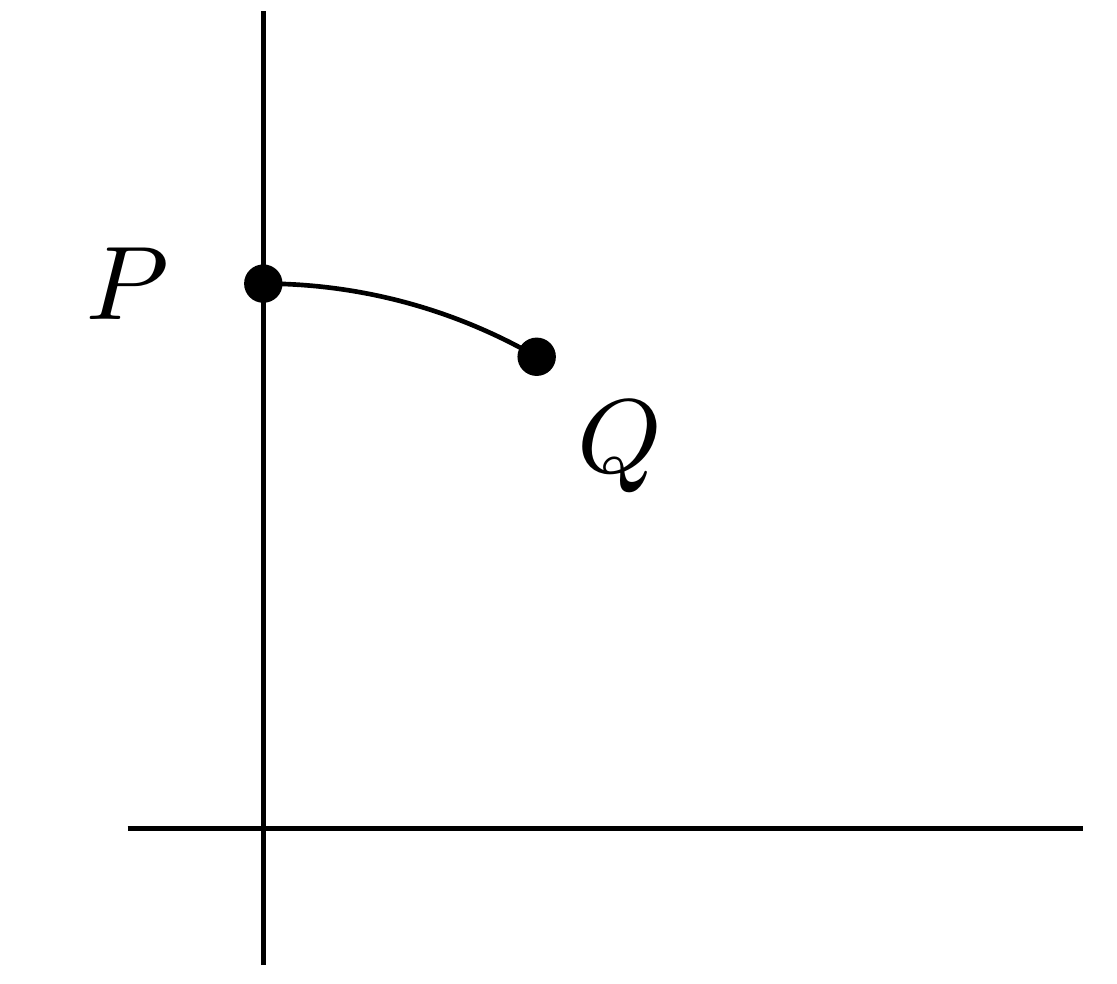
\includegraphics[width=5cm]{assets/circle-segment.png}
        \centering
    \end{figure}
    có nhóm con ổn định đẳng cấu lần lượt với $\Z/2, \Z/4$ và $\Z/6$.
\end{proposition}

\startproof
Do
$$
    \begin{aligned}
        \frac{ai+b}{ci+d} =i & \ \Leftrightarrow\ b+ia=-c+id             \\
                             & \ \Leftrightarrow\  b=-c\ \text{ và } a=d
    \end{aligned}
$$
và $ad - bc = 1$ nên $a^2 + b^2 = 1$. Bằng cách xét 2 trường hợp $a = 0$ hay $b = 0$, ta có $4$ ma trận tương ứng nhóm con cyclic cấp $4$ sinh bởi $S =\begin{pmatrix}
        0 & -1 \\
        1 & 0
    \end{pmatrix}$. Vậy $\langle S \rangle$ là nhóm con cố định $P$. Tương tự ta cũng xét
$$
    \begin{aligned}
        \frac{ae^{i\pi /3} +b}{ce^{i\pi /3} +d} =e^{i\pi /3} & \ \Leftrightarrow\ \left(\frac{a}{2} +b\right) +ia\frac{\sqrt{3}}{2} =\left( -\frac{c}{a} +\frac{d}{a}\right) +i\frac{\sqrt{3}}{2}( c+d) \\
                                                             & \ \Leftrightarrow\ a+2b=d-c\text{ và } a=c+d                                                                                             \\
                                                             & \ \Leftrightarrow\ b=-c\text{ và } a( a-c) +c^{2} =1.
    \end{aligned}
$$
Giải phương trình $a^2-ca+(c^2-1)=0$, ta có $c^2 - 4(c^2-1) \geq 0$ và do đó $|c| \leq \frac{2}{\sqrt{3}} \approx 1.154$. Suy ra ta có các khả năng $c = 0,\ c=1$ hay $c=-1$. Mỗi giá trị của $c$ lại cho ra $2$ giá trị $a$ tương ứng. $b$ và $d$ thì phụ thuộc vào $c$ và $a$. Từ đó ta có $6$ ma trận tương ứng và chúng là các phần tử của nhóm con cấp $6$ sinh bởi $R = \begin{pmatrix}
        1 & -1 \\
        1 & 0
    \end{pmatrix}$. Suy ra $\langle R \rangle$ là nhóm con cố định $Q$.

Nhóm con ổn định $Y$ phải nằm trong phần giao $\langle S \rangle \cap \langle R \rangle$ và do đó phải bằng $\{I,-I\}$ vì $I$ và $-I$ đều là các tác động tầm thường.\qed

\begin{theorem}
    $X = SL_2(\Z) \cdot Y$ là cây và $Y$ là miền cơ bản dưới tác động của $SL_2(\Z)$ lên $X$. Do đó ta có
    $$
        SL_2(\Z) \cong \Z/4 *_{\Z/2} \Z/6.
    $$
\end{theorem}

\startproof Đầu tiên ta cần chứng tỏ rằng $X$ là nhận dạng của đồ thị, thật vậy ta sẽ chỉ ra rằng dưới tác động của $\gamma$ thì $Y$ chỉ có thể giao với $\gamma (Y)$ tại $\gamma(P)$ hoặc $\gamma(Q)$. Giả sử $\gamma(Y) \cap Y \neq \varnothing$, dựa trên Bổ đề $\ref{lem:fundamental-domain}$, ta chia ra 2 trường hợp.

Nếu $c^2 \neq d^2$, ta có $\frac{1}{|c^2-d^2|} = 1$, vậy $c$ hoặc $d$ bằng $0$ và tâm $\mu = (ac-bd)/(c^2-d^2)$ phải bằng $0$ hoặc $1$. Nếu $\mu = 0$ thì $\gamma$ hoặc $\gamma$ là phép tịnh tiến, nghĩa là phải bằng $\pm I$, hoặc $\gamma = S$ nếu $a = 0$ ($S$ là phép phản xạ $Y$ qua trục $y$  do $S(Y) = -\bar{Y}$). Nếu $\mu = 1$, $d = 0$, $ac = 1$ thì $\gamma = \pm R$ (cố định $Q$).

Nếu $c^2 = d^2 = 1$ thì phần thực phải bằng $1/2$, do đó $a \in \{0,1,-1\}$. Nếu $a = 0$ thì $\gamma = \pm R^2$ (cố định $Q$) và với $a = \pm$ thì phần giao phải bằng rỗng (mâu thuẫn).

$SL_2(\Z)$ được sinh bởi $S$ và $R$ theo Mệnh đề \ref{prop:SR-gen-sl2}, do đó bất kì tác động $\gamma \in SL_2(\Z)$ lên $Y$ đều tương ứng với một chuỗi tác động bởi $S$ và $R$. Ta có $Y$ liên thông với $S(Y)$ và $R(Y)$ và do đó $Y' = S(Y) \cup Y \cup R(Y)$ liên thông, tương tự ta cũng có $Y'' = S(Y') \cup Y' \cup R(Y')$ liên thông. Cứ tiếp tục quá trình trên ta có $X$ là một đồ thị liên thông.

Cuối cùng, ta có $C = S^1 \cap \HC$ chỉ cắt $X$ tại điểm $P=i$ trên trục $y$, suy ra cạnh duy nhất của $X$ cắt trục $y$ là $Y$ và $S(Y)$. Hơn nữa bất kì đường đi nào trong $X$ đều có thể tịnh tiến để cắt trục $y$, do đó nếu $X$ chứa chu trình thì $X$ phải cắt trục $y$ 2 lần, điều này là mâu thuẫn và do đó $X$ là cây. Theo Định lí \ref{thm:bass-serre-fund} ta có điều phải chứng minh. \qed

\begin{figure}[H]
    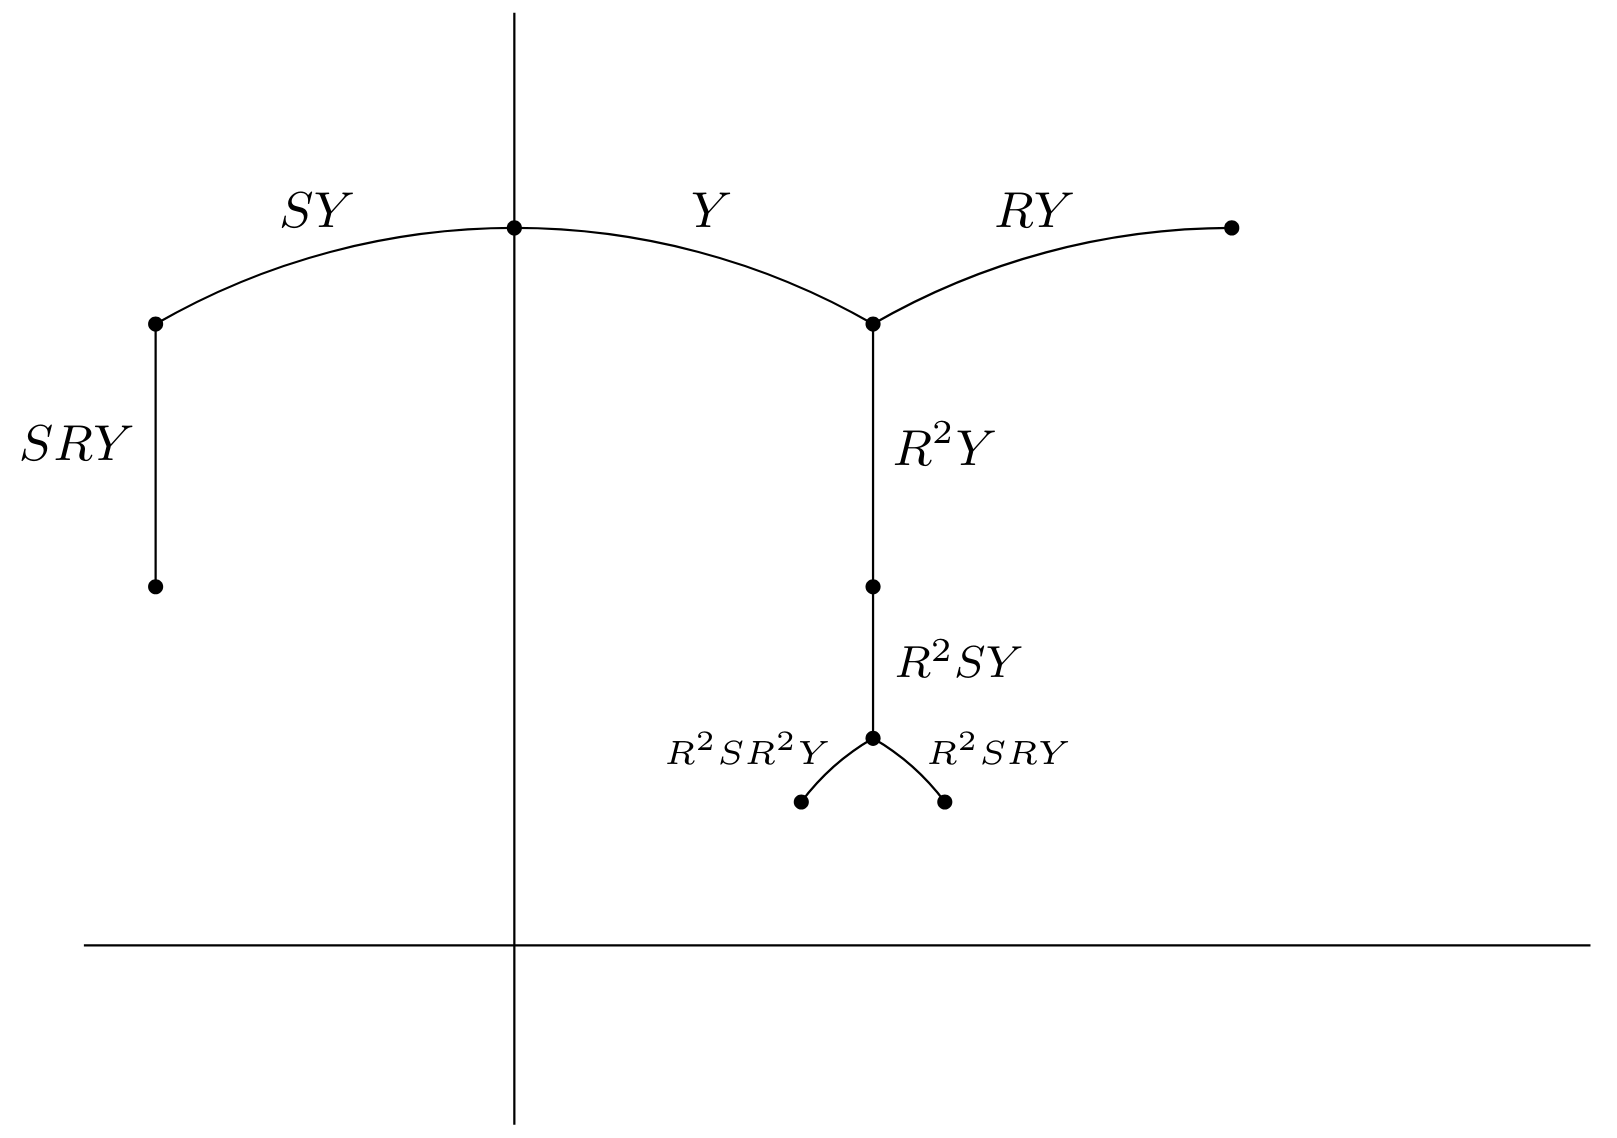
\includegraphics[width=13cm]{assets/sl2z-tree.png}
    \centering
\end{figure}

\begin{corollary}\label{cor:sl2z-presentation}
    Từ phân tích amalgam trên, ta có biểu diễn
    $$
        SL_2(\Z) = \langle R,S\ |\ R^6 = S^4 = 1, R^3 = S^2 \rangle.
    $$
    Ngoài ra với nhóm tuyến tính xạ ảnh đặc biệt $PSL_2(\Z) = SL_2(\Z) / \{\pm I\}$ thì ta cũng có phân tích
    $$
        PSL_2(\Z) \cong \Z/2 * \Z/3.
    $$
    và biểu diễn
    $$
        PSL_2(\Z) = \langle R, S \rangle = \langle R^3 = S^2 = 1 \rangle = \langle S, T\ |\ S^2 = (ST)^3 = 1 \rangle.
    $$
\end{corollary}

\section{Đối đồng điều của $SL_2(\Z)$}
Để tránh nhầm lẫn với phép cộng trong vành nhóm, trong phần này ta kí hiệu $C_n$ viết theo lối nhân cho nhóm cyclic cấp $n$.

\begin{theorem}
    $$
        H^n(SL_2(\Z);\Z) = \begin{cases}
            \Z,      & n = 0               \\
            0,       & n \text{ lẻ}        \\
            \Z / 12, & n > 0 \text{ chẵn}.
        \end{cases}
    $$
\end{theorem}
\vspace{4mm}
\startproof
Gọi $r,s$ và $t$ lần lượt là phần tử sinh của $C_2$, $C_4$ và $C_6$. Ta biết rằng phân tích amalgam của $SL_2(\Z)$ được biểu diễn thông qua các đồng cấu
$$
    \alpha_1: C_2 \rightarrow C_4,\ r \mapsto s^2\ \text{và}\ \alpha_2: C_2 \rightarrow C_6,\ r \mapsto t^3
$$
Sử dụng phép giải cho $C_2$ và $C_4$ mà ta đã đưa ra trong lúc tính đối đồng điều cho nhóm cyclic
$$
    \begin{tikzcd}
        \cdots \arrow[r, "r-1"] & \Z C_2 \arrow[rr, "1+r"] \arrow[d, "f_2"] &  & \Z C_2 \arrow[r, "r-1"] \arrow[d, "f_1"] & \Z C_2 \arrow[r, "\varepsilon_1"] \arrow[d, "f_0"] & \Z \arrow[r] \arrow[d, "\id"] & 0 \\
        \cdots \arrow[r, "s-1"] & \Z C_4 \arrow[rr, "1+s+s^2+s^3"]          &  & \Z C_4 \arrow[r, "s-1"]                  & \Z C_4 \arrow[r, "\varepsilon_2"]                  & \Z \arrow[r]                 & 0
    \end{tikzcd}
$$
ta mong muốn xây dựng ánh xạ dây chuyền $f = \{f_n: \Z C_2 \rightarrow \Z C_4 \}$ giữa hai phép giải, trong đó $f_0$ là mở rộng tuyến tính lên vành nhóm của đồng cấu $\alpha_1: C_2 \rightarrow C_4$. Để ý rằng $f_n$ được xác định duy nhất thông qua $f_n(1)$.

Với $n$ chẵn, giả sử tính giao hoán của biểu đồ trên, ta có
\begin{equation}
    (1+s+s^2+s^3)f_{n+1}(1) = f_n((1+r)\cdot 1) = f_n(1+\alpha_1(r)) = (1+s^2) f_n(1).\label{eq:fn_commute}
\end{equation}
Tác động $s-1$ vào ta được
$$
    0 = (s-1)(1+s+s^2+s^3)f_{n+1}(1) = (s-1)(1+s^2)f_n(1) = (-1+s-s^2+s^3)f_n(1).
$$
Do đó ta có thể chọn $f_n(1) = 1+s$ để thỏa đẳng thức trên. Bây giờ $\ref{eq:fn_commute}$ trở thành thành
$$
    (1+s+s^2+s^3)f_{n+1}(1) = (1+s^2)(1+s) = 1+s+s^2+s^3.
$$
Vậy bằng cách chọn $f_{n+1}(1) = 1$, ta có $f$ là một ánh xạ dây chuyền như mong muốn.

Tiếp theo, ta tác động lần lượt $\Hom_{C_2}(-, \Z)$ và $\Hom_{C_2}(-, \Z)$ vào hai phép giải trên
$$
    \begin{tikzcd}
        \cdots & \Z \arrow[l, "2"']                     & \Z \arrow[l, "0"']                     & \Z \arrow[l, "2"']                     & \Z \arrow[l, "0"']                     \\
        \cdots & \Z \arrow[l, "2"'] \arrow[u, "f_3^*"'] & \Z \arrow[u, "f_2^*"'] \arrow[l, "0"'] & \Z \arrow[l, "4"'] \arrow[u, "f_1^*"'] & \Z \arrow[l, "0"'] \arrow[u, "f_0^*"']
    \end{tikzcd}
$$
Trong đó $f_n^*(1) = 2$ nếu $n$ chẵn và $f_n^*(1) = 1$ nếu $n$ lẻ. Ta biết rằng
$$
    H^n(C_k;\Z) = \begin{cases}
        \Z,  & n = 0               \\
        0,   & n \text{ lẻ}        \\
        C_k, & n > 0 \text{ chẵn}.
    \end{cases}
$$
Từ đó $\{f^*_n\}$ cảm sinh ra đồng cấu $\alpha_1^*: H^n(C_4; \Z) \rightarrow H^n(C_6;\Z)$ là đồng cấu đồng nhất nếu $n = 0$, là đồng cấu tầm thường nếu $n > 0$ lẻ và là đồng cấu biến $s \mapsto r$ nếu $n > 0$ chẵn.

Tương tự ta cũng xây dựng được đồng cấu $\alpha^*_2: H^n(C_6; \Z) \rightarrow H^n(C_2;\Z)$ xác định như trên, với $t \mapsto r$ trong trường hợp $n > 0$ chẵn.

Hai đồng cấu này cảm sinh duy nhất từ $\alpha_1$ và $\alpha_2$, do đó chúng cũng là đồng cấu nối trong dãy khớp dài ở Mệnh đề \ref{prop:long-seq-amalgam}
$$
    \cdots \xrightarrow{} H^{n-1}(C_2) \xrightarrow{\psi} H^n(SL_2(\Z)) \xrightarrow{\varphi} H^n(C_4) \oplus H^n(C_6) \xrightarrow{\alpha_1^* + \alpha_2^*} H^n(C_2) \xrightarrow{} \cdots
$$
trong đó $\alpha_1^* + \alpha_2^*: (a,b) \mapsto a + b$ là toàn ánh với mỗi $n$. Do đó $\psi = 0$ và $\varphi$ là đơn cấu.

Dãy khớp tại $n = 0$ có dạng
$$
    0 \xrightarrow{} H^0(SL_2(\Z)) \xrightarrow{\varphi} \Z \oplus \Z \xrightarrow{} \Z \xrightarrow{} \cdots
$$
Suy ra $H^0(SL_2(\Z)) \cong \im(\varphi) = \ker(\alpha_1^* + \alpha_2^*) = \langle (1,-1) \rangle \cong \Z$. Với $n > 0$ chẵn, ta có
$$
    \cdots \xrightarrow{} H^n(SL_2(\Z)) \xrightarrow{\varphi} C_4 \oplus C_6 \xrightarrow{} C_2 \xrightarrow{} \cdots
$$
Để ý rằng nếu ta viết $C_4$ và $C_6$ theo dạng nhóm cộng modulo thì $\ker(\alpha_1^* + \alpha_2^*)$ là tập các cặp $(a,b)$ sao cho $a$ và $b$ cùng chẵn hoặc cùng lẻ, nghĩa là nhóm có cấp $12$. Hơn nữa nó còn là nhóm cyclic sinh bởi $\langle (1,1) \rangle$. Do đó $H^n(SL_2(\Z)) \cong \im(\varphi) = \ker(\alpha_1^* + \alpha_2^*) \cong C_{12}$. Với $n$ lẻ thì ta có
$$
    \cdots \xrightarrow{} H^{n-1}(C_2) \xrightarrow{} H^n(SL_2(\Z)) \xrightarrow{\varphi} 0 \xrightarrow{} \cdots
$$
do đó $H^n(SL_2(\Z)) = 0$ vì $\varphi$ là đơn cấu. \qed

\begin{corollary}
    Từ Định lí hệ số phổ dụng \ref{cor:universal-coef}, ta cũng tính được đồng điều thứ $n$ của $SL_2(\Z)$ cho bởi
    $$
        H_n(SL_2(\Z);\Z) = \begin{cases}
            \Z,      & n = 0               \\
            \Z / 12, & n \text{ lẻ}        \\
            0,       & n > 0 \text{ chẵn}.
        \end{cases}
    $$
\end{corollary}
\pagebreak
\chapter{Đồng điều thứ nhất của $SL_2(\Z[1/m])$}

Ở chương này, dựa trên kết quả Carl-Fredrik \cite{CarlAbelSL2}, ta sẽ tính đồng điều thứ nhất của nhóm $SL_2(\Z[1/m])$ với $m$ bất kì thông qua abel hóa (Định lí \ref{thm:first-homology}).

Cho $m \geq 1$, định nghĩa nhóm
$$
    \mathcal{H}_m = \langle x,y\ |\ x^m y x^m = yx^my, y^mxy^m = xy^mx, (x^2y^m)^4 = 1 \rangle.
$$
Ta bắt đầu phần này với một quan sát.

\begin{proposition}
    $$
        \mathcal{H}_1 \cong SL_2(\Z).
    $$
\end{proposition}
\startproof Trước tiên ta ghi lại
\begin{equation}\label{eq:h1-presentation}
    \mathcal{H}_1 = \langle x,y\ |\ xyx = yxy, (x^2y)^4 = 1 \rangle
\end{equation}
Ta sẽ chứng tỏ biểu diễn trên tương đương với biểu diễn ta đưa ra cho $SL_2(\Z)$ ở Hệ quả \ref{cor:sl2z-presentation}
$$
    SL_2(\Z) = \langle R,S\ |\ R^6 = S^4 = 1, R^3 = S^2 \rangle.
$$
Ta có $(x^2y)^4 = x(xyx)(xyx)(xyx)xy = x(yxy)(yxy)(yxy)xy = (xy)^6$. Vậy bằng cách đặt $r = xy$, $s = x^2y$, ta sẽ đưa về được biểu diễn mong muốn, thật vậy
\begin{align*}
    r^3 = s^2 \Longleftrightarrow x^2yx^2y = xyxyxy \Longleftrightarrow xyx = yxy.
\end{align*}
Suy ra biểu diễn \ref{eq:h1-presentation} tương đương với $\langle r,s\ |\ r^6 = s^4 = 1, r^3 = s^2 \rangle \cong SL_2(\Z)$.\qed

\begin{lemma}[\cite{MennickeIhara}]\label{lem:gen-sl2-1m}
    $SL_2(\Z[1/m])$ được sinh bởi ba ma trận sau
    $$
        A = \begin{pmatrix}
            1 & 0 \\
            1 & 1
        \end{pmatrix},\enskip
        B = \begin{pmatrix}
            0  & 1 \\
            -1 & 0
        \end{pmatrix},\enskip
        U_m = \begin{pmatrix}
            m & 0   \\
            0 & 1/m
        \end{pmatrix}.
    $$
\end{lemma}
% \startproof Xét $\gamma = \begin{pmatrix}
%         a & b \\
%         c & d
%     \end{pmatrix} \in SL_2(\Z[1/m])$

\begin{lemma}\label{lem:surject-phi-m}
    Với $m \geq 1$, ánh xạ $\varphi_m: \mathcal{H}_m \rightarrow SL_2(\Z[1/m])$ xác định bởi
    $$
        \varphi_m(x) = A = \begin{pmatrix}
            1 & 0 \\
            1 & 1
        \end{pmatrix} \enskip\text{và}\enskip
        \varphi_m(y) = Q_m = \begin{pmatrix}
            1 & -1/m \\
            0 & 1
        \end{pmatrix}
    $$
    là toàn cấu.
\end{lemma}
\startproof Đầu tiên để kiểm tra tính đồng cấu, ta cần kiểm tra ảnh của mọi quan hệ trên $\mathcal{H}_m$ phải bảo toàn qua $\varphi_m$, thật vậy
\begin{align*}
    A^m Q_m A^m = \begin{pmatrix}
                      0 & -1/m \\
                      m & 0
                  \end{pmatrix} = Q_m A^m Q_m. \\
    Q_m^m A Q_m^m = \begin{pmatrix}
                        0 & -1 \\
                        1 & 0
                    \end{pmatrix} = A Q_m^m A. \\
    A^2Q_m^m = \begin{pmatrix}
                   1 & -1 \\
                   2 & -1
               \end{pmatrix}\text{ là phần tử cấp 4}.
\end{align*}
Để chứng tỏ $\varphi_m$ toàn ánh, để ý rằng
% $SL_2(\Z[1/m])$ được sinh bởi ba ma trận
% $$
%     A = \begin{pmatrix}
%         1 & 0 \\
%         1 & 1
%     \end{pmatrix},\enskip
%     B = \begin{pmatrix}
%         0  & 1 \\
%         -1 & 0
%     \end{pmatrix},\enskip
%     U_m = \begin{pmatrix}
%         m & 0   \\
%         0 & 1/m
%     \end{pmatrix}.
% $$
% Hơn nữa
$$
    B = A^{-1}Q_m^{-m}A^{-1}\enskip\text{và}\enskip U_m = B^{-1}Q_m^{-1}A^{-m}Q_m^{-1},
$$
Kết hợp với Bổ đề \ref{lem:gen-sl2-1m} ta suy ra được $A = \varphi_m(x)$ và $U_m = \varphi_m(y)$ sinh ra $SL_2(\Z[1/m])$. Vậy $\varphi_m$ toàn cấu.\qed

\begin{theorem}\label{thm:abel-sl2-1m}
    Với $m \geq 1$, ta có
    $$
        H_1(SL_2(\Z[1/m])) = (\mathcal{H}_m)^{\ab} \cong \begin{cases}
            1     & \text{nếu } 6\ |\ m,                           \\
            \Z/3  & \text{nếu } 2\ |\ m \text{ và } \gcd(m,3) = 1, \\
            \Z/4  & \text{nếu } 3\ |\ m \text{ và } \gcd(m,2) = 1, \\
            \Z/12 & \text{nếu } \gcd(m,6) = 1.
        \end{cases}
    $$
\end{theorem}
\startproof Bằng cách thêm quan hệ giao hoán cho $\mathcal{H}_m$ ta được
\begin{align*}
    (\mathcal{H}_m)^{\ab} & = \langle x,y\ |\ x^m = y,\ y^m = x,\ x^8y^{4m} = 1,\ xy=yx \rangle \\
                          & = \langle x\ |\ x^{m^2-1} = 1,\ x^{4m^2+8} = 1 \rangle              \\
                          & \cong \Z/\gcd(m^2-1, 4m^2+8).
    % (\mathcal{H}_m)^{\ab} \cong \Z/\gcd(m^2+1, 12m, 4m^2+8).
\end{align*}
Đặt $G_m = SL_2(\Z[1/m])^{\ab}$. Từ Bổ đề \ref{lem:surject-phi-m} suy ra $\varphi_m$ cảm sinh một toàn cấu $\varphi_m^{\ab}: (\mathcal{H}_m)^{\ab} \rightarrow G_m$. Nếu $6\ |\ m$ thì $(\mathcal{H}_m)^{\ab} = 1$, dẫn đến $G_m = 1$. Nếu $2\ |\ m$ và $\gcd(m,3)=1$ thì $|G_m| \leq 3$, tuy nhiên trong trường hợp này ta có toàn cấu từ $SL_2(\Z[1/m])$ vào $SL_2(\Z/3)$ (là nhóm có abel hóa bằng $\Z/3$), do đó $G_m \cong \Z/3$. Nếu $3\ |\ m$ và $\gcd(2,m)=1$ thì $|G_m| \leq 4$, tuy nhiên lúc này ta lại có toàn cấu từ $SL_2(\Z[1/m])$ vào $SL_2(\Z/4)$ (là nhóm có abel hóa bằng $\Z/4$), do đó $|G_m| = \Z/4$. Cuối cùng, nếu $\gcd(m,6) = 1$ thì khi đó $|G_m| \leq 12$, kết hợp hai lập luận trên ta suy ra $G_m \cong \Z/4 \times \Z/3 \cong \Z/12$.\qed
\pagebreak
\chapter{Đối đồng điều của $SL_2(\Z[1/p])$}
Đối đồng điều của $SL_2(\Z[1/p])$ với $p$ nguyên tố đã được Adem và Naffah tính triệt để vào 1998 \cite{AdemSL2}. Trong chương này, tôi sẽ trình bày lại công trình nêu trên của hai tác giả.

Nhắc lại Hệ quả \ref{cor:amalgam-sl2-1p}, ta có phân tích amalgam
$$
    SL_2(\Z[1/p]) \cong SL_2(\Z) *_{\Gamma_0(p)} SL_2(\Z),
$$
trong đó $\Gamma_0(p)$ là nhóm con đồng dư Hecke của $SL_2(\Z)$. Ta đã tính được đối đồng điều của $SL_2(\Z)$ từ chương trước, bước tiếp theo ta cần tính đối đồng điều của nhóm con đồng dư $\Gamma_0(p)$.

\section{Phân tích lớp kề}
Ta kí hiệu $C_2, C_4$ và $C_6$ là các nhóm con cyclic của $SL_2(\Z)$ lần lượt sinh bởi ma trận $a_2, a_4$ và $a_6$ cho bởi
$$
    a_{2} =\begin{pmatrix}
        -1 & 0  \\
        0  & -1
    \end{pmatrix} ,\ a_{4} =\begin{pmatrix}
        0 & -1 \\
        1 & 0
    \end{pmatrix} ,\ a_{6} =\begin{pmatrix}
        0 & -1 \\
        1 & 1
    \end{pmatrix}.
$$
Xét $G = SL_2(\F_p)$ và
$$
    B = \left\{ \begin{pmatrix}
        * & * \\
        0 & *
    \end{pmatrix} \in SL_2(\F_p) \right\}
$$
là nhóm con của $G$. Ta dễ dàng kiểm tra được tập các lớp kề phải $B \setminus G$ có phân tích
$$
    B \setminus G = B a_4 \sqcup \left( \bigsqcup_{x \in \F_p} B \begin{pmatrix}
        1 & 0 \\
        x & 1
    \end{pmatrix} \right).
$$
Do $a_2$ nằm trong tâm của $G$ nên ta có phân tích lớp kề đôi cho $G$ dùng $B$ và $C_2$ như sau
$$
    G = B a_4 C_2 \sqcup \left( \bigsqcup_{x \in \F_p} B \begin{pmatrix}
        1 & 0 \\
        x & 1
    \end{pmatrix} C_2 \right).
$$
Áp dụng công thức lớp kề đôi, ta được
$$
    \Z[G/C_2]_{|B} \cong (\Z[B/C_2])^{p+1}.
$$
Tiếp theo ta xét lớp kề đôi của $G$ dùng $C_4$. Để ý rằng
$$
    \begin{pmatrix}
        1 & 0 \\
        x & 1
    \end{pmatrix}\begin{pmatrix}
        0 & -1 \\
        1 & 0
    \end{pmatrix} =\begin{pmatrix}
        0 & -1 \\
        1 & -x
    \end{pmatrix} \text{ và } \begin{pmatrix}
        0 & -1 \\
        1 & -x
    \end{pmatrix}\begin{pmatrix}
        1   & 0 \\
        1/x & 1
    \end{pmatrix} =\begin{pmatrix}
        -1/x & -1 \\
        0    & -x
    \end{pmatrix}.
$$
Từ đây ta kết luận, trong trường hợp $x \neq -1/x$ hay $x \neq 0$, thì
$$
    B\begin{pmatrix}
        1 & 0 \\
        x & 1
    \end{pmatrix}\begin{pmatrix}
        0 & -1 \\
        1 & 0
    \end{pmatrix} =B\begin{pmatrix}
        1    & 0 \\
        -1/x & 1
    \end{pmatrix}.
$$
Suy ra
$$
    B\begin{pmatrix}
        1 & 0 \\
        x & 1
    \end{pmatrix} C_{4} =B\begin{pmatrix}
        1 & 0 \\
        x & 1
    \end{pmatrix} \sqcup B\begin{pmatrix}
        1    & 0 \\
        -1/x & 1
    \end{pmatrix}\text{ và } Ba_4C_4 = B \sqcup B a_4.
$$
Đối với cả hai trường hợp, hai lớp kề bị hoán vị bởi ma trận $a_4$. Trong trường hợp $x^2+1=0$, lớp kề bị cố định bởi tác động này và do đó bằng với lớp kề đôi tương ứng. Nhắc lại một kết quả sơ cấp rằng đa thức $t^2+1$ có nghiệm trong $\F_p$ khi và chỉ khi $p \equiv 1 \mmod 4$. Điều này cộng với công thức lớp kề đôi ta được
$$
    \Z[G/C_4]_{|B} \cong \Z[B/s_1 C_4 s_1^{-1}] \oplus \Z[B/s_2 C_4 s_2^{-1}] \oplus (\Z[B/C_2])^{(p-1)/2}
$$
nếu $p \equiv 1\ \operatorname*{mod}\ 4$, trong đó trong đó $s_1,s_2$ ứng với hai nghiệm của đa thức $x^2+1=0$. Và với các trường hợp còn lại thì
$$
    \Z[G/C_4]_{|B} \cong (\Z[B/C_2])^{(p-1)/2}.
$$

Với $C_6$ ta cần nhìn vào tác động của ma trận cấp $3$, $\begin{pmatrix}
        0  & 1  \\
        -1 & -1
    \end{pmatrix}$ lên lớp kề đôi. Trong trường hợp này thì quỹ đạo của tác động trên có dạng
$$
    B\begin{pmatrix}
        1 & 0 \\
        x & 1
    \end{pmatrix},\enskip
    B\begin{pmatrix}
        1       & 0 \\
        1/(1-x) & 1
    \end{pmatrix},\enskip
    B\begin{pmatrix}
        1       & 0 \\
        (x-1)/x & 1
    \end{pmatrix}
$$
trong đó $x \neq 1$. Lớp kề bị cố định khi và chỉ khi $x^2 - x + 1 = 0$. Nếu $p > 3$, đa thức có nghiệm trong $\F_p$ khi và chỉ khi $p \equiv 1 \mmod 3$. Nếu $x=1$, lớp kề cho ta các quỹ đạo
$$
    B,\enskip
    B\begin{pmatrix}
        1 & 0 \\
        1 & 1
    \end{pmatrix},\enskip
    Ba_4.
$$
Từ đó ta có phân tích
$$
    \Z[G/C_6]_{|B} \cong \Z[B/s_1C_6s_1^{-1}] \oplus \Z[B/s_2 C_6 s_2^{-1}] \oplus \Z[B/C_2]^{(p-1)/3} \text{ nếu } p \equiv 1 \mmod 3
$$
và
$$
    \Z[G/C^6]_{|B} \cong \Z[B/C_2]^{(p+1)/3} \text{ trong trường hợp còn lại}.
$$
\section{Đối đồng điều thứ nhất của $\Gamma_0(p)$}
Nhắc lại chương 1 thì $SL_2(\Z)$ tác động lên cây $X$ có các nhóm con ổn định hữu hạn. Ta có nhóm con đồng dư chính $\Gamma(p)$ tự do xoắn nên tác động tự do lên X, từ đó cảm sinh ra tác động của $G = SL_2(\F_p)$ lên đồ thị hữu hạn $X/\Gamma(p)$. Nhóm con ổn định của tác động này chính là $C_4$ và $C_6$ đối với đỉnh và $C_2$ đối với cạnh của miền cơ bản. Trước tiên ta sẽ đi mô tả cấu trúc của không gian phân loại $B\Gamma_0(p)$ của $\Gamma_0(p)$.
% Bằng phép chiếu $\pi: \Gamma_0(p) \rightarrow B$, $\Gamma_0(p)$ tác động chéo lên $EB \times X$ với nhóm con ổn định tầm thường. Do không gian này co rút được, không gian quỹ đạo dưới tác động này có cùng kiểu đồng luân với không gian phân loại $B\Gamma_0(p)$, và do đó $B\Gamma_0(p) \cong (EB \times T/\Gamma(p))/B$.

\begin{proposition}
    Xét $EB$ là không gian co rút được sao cho tác động cho bởi $B$ là tác động tự do. Khi đó
    $$
        B\Gamma_0(p) \cong (EB \times T/\Gamma(p))/B.
    $$
\end{proposition}

\startproof Xét dãy khớp ngắn cho bởi
$$
    1 \rightarrow \Gamma(p) \rightarrow \Gamma_0(p) \rightarrow B \rightarrow 1.
$$
Sử dụng phép chiếu $\pi: \Gamma_0 \rightarrow B$, ta định nghĩa tác động chéo của $\Gamma_0(p)$ lên $EB \times X$ cho bởi
$$
    g(x,y) = (x(\pi(g))^{-1}, gy).
$$
Vì $B$ tác động tự do lên $EB$ nên tác động ta đưa ra cũng tự do. Hơn nữa $EB \times X$ cũng là không gian co rút được nên không gian quỹ đạo $(EB \times X) / \Gamma_0(p)$ tương đương đồng luân với không gian phân loại $B\Gamma_0(p)$. Cuối cùng ta có
$$
    (EB \times X) / \Gamma_0(p) \cong (EB \times X/\Gamma(p))/B.
    \eqno\qed
$$

% \begin{proposition}
Gọi $C^*$ là đối phức ô tương ứng với phức $B$-CW của cây $T/\Gamma(p)$, từ các lập luận trên ta suy ra được
$$
    C^0 \cong \Z[G/C_4]_{|B} \oplus \Z[G/C_6]_{|B} \text{ và } C^1 \cong \Z[G/C_2]_{|B}.
$$

Lúc này dãy phổ đẳng biến theo lọc thứ 2 được mô tả ở Định lí \ref{thm:equiv-spec} hội tụ về $H^*(\Gamma_0(p))$, với $E_1^{pq} \cong H^q(B,C^p)$. Ngoài ra $E_2^{pq} = 0$ ngoại trừ $p=0,1$, do đó theo Mệnh đề \ref{prop:spec-exact} ta có dãy khớp
$$
    0 \rightarrow E_2^{1,n-1} \rightarrow H^n(\Gamma_0(p)) \rightarrow E_2^{0,n} \rightarrow 0.
$$
Từ đó ta có dãy khớp dài
\begin{equation}\label{eq:long-gamma-p}
    \cdots \rightarrow H^i(\Gamma_0(p)) \rightarrow H^i(B,C^0) \rightarrow H^i(B,C^1) \rightarrow H^{i+1}(\Gamma_0(p); \Z) \rightarrow \cdots,
\end{equation}
trong đó đồng cấu ở giữa là đồng cấu cảm sinh từ đồng cấu biên của $C^*$.

\begin{proposition}\label{prop:first-cohom-congurence}
    $H^1(\Gamma_0(p); \Z) \cong \Z^{N(p)}$, trong đó
    $$
        N(p) = \begin{cases}
            (p-7)/6, & \text{nếu } p \equiv 1 \mmod 12,  \\
            (p+1)/6, & \text{nếu } p \equiv 5 \mmod 12,  \\
            (p-1)/6, & \text{nếu } p \equiv 7 \mmod 12,  \\
            (p+7)/6, & \text{nếu } p \equiv 11 \mmod 12.
        \end{cases}
    $$
\end{proposition}

\startproof Đoạn đầu của dãy khớp \ref{eq:long-gamma-p} có dạng
$$
    0 \rightarrow \Z \rightarrow (C^0)^B \rightarrow (C^1)^B \rightarrow H^1(\Gamma_0(p); \Z) \rightarrow H^1(B; C^0) \rightarrow \cdots
$$
Sử dụng công thức lớp ghép đôi và Mệnh đề \ref{prop:cohom-coef-prod} ta được
$$
    H^1(B;C^0) \cong H^1(B; \Z[G/C_4]_{|B}) \oplus H^1(B;\Z[G/C_6]_{|B}).
$$
Trong trường hợp $p \equiv 1 \mmod 4$, cũng từ Mệnh đề \ref{prop:cohom-coef-prod} ta suy ra
$$
    H^1(B;\Z[G/C_4]_{|B}) \cong H^1(B;\Z[B/s_1C_4s_1^{-1}]) \oplus H^1(B;B/s_2C_4s_2^{-1}) \oplus H^1(B;\Z[B/C_2]^{(p-1)/2}).
$$
Tính tiếp cho $H^1(B;\Z[G/C_2]_{|B})$ ta được
$$
    H^1(B;\Z[B/C_2]^{(p-1)/2}) \cong \bigoplus_{i=1}^{(p-1)/2} H^1(B;\Z[B/C_2]),
$$
lúc này theo bổ đề Shapiro
\begin{align*}
    H^1(B;\Z[B/C_2]^{(p-1)/2}) & \cong \bigoplus_{i=1}^{(p-1)/2} H^1(B;\Ind_{C_2}^B\Z) \\
                               & \cong \bigoplus_{i=1}^{(p-1)/2} H^1(C_2;\Z)           \\
                               & \cong 0.
\end{align*}
Tiếp tục ta có
\begin{align*}
    H^1(B;\Z[B/s_1C_4s_1^{-1}]) & \cong H^1(B;\Ind_{s_1C_4s_1^{-1}}\Z) \\
                                & \cong H^1(s_1C_4s_1^{-1}; \Z)        \\
                                & \cong H^1(C_4;\Z)                    \\
                                & \cong 0.
\end{align*}
Điều này dẫn đến $H^1(B;\Z[G/C_4])$ cũng tầm thường. Sử dụng lập luận trên cho các trường hợp còn lại ta được $H^1(B,C^0) \cong 0$.

\section{Đối đồng điều của nhóm con đồng dư $\PGam_0(p)$}
\begin{lemma}
    Nhắc lại sự phân tính ở Hệ quả \ref{cor:sl2z-presentation}
    $$
        PSL(2,\Z) \cong \Z/2 * \Z/3.
    $$
    Theo dãy phổ đẳng biến ta được dãy khớp dài
    \begin{equation}\label{eq:long-equivariant}
        \cdots \rightarrow H^i(\PGam_0(p);\Z) \rightarrow H^i(PB; PC^0) \rightarrow H^i(PB;PC^0) \rightarrow H^{i+1}(\PGam_0(p);\Z) \rightarrow \cdots
    \end{equation}
\end{lemma}

\begin{proposition}
    $H^1(\PGam_0(p);\Z) \cong H^1(\Gamma_0(p);\Z)$.
\end{proposition}
\startproof Phần đầy của dãy khớp \ref{eq:long-equivariant} có dạng
$$
    0 \rightarrow (PC^0)^{PB} \rightarrow (PC^1)^{PB} \rightarrow H^1(\PGam_0(p);\Z) \rightarrow H^1(PB, PC^0) \rightarrow \cdots
$$
Theo Mệnh đề \ref{prop:first-cohom-congurence} thì $H^1(PB;PC^0) = 0$. Để ý rằng $(PC^0)^{PB}$ và $(PC^1)^{PB}$ có hạng bằng nhau, $(PC^1)^{PB}$ và $(C^1)^B$ có hạng bằng nhau, do đó ta có điều phải chứng minh.\qed

\begin{proposition}
    Với số nguyên $i \geq 1$, ta có
    $$
        H^{2i}(\PGam_0(p);\Z) \cong \begin{cases}
            \Z/6 \oplus \Z/6 & \text{nếu } p \equiv 1 \mmod 12,  \\
            \Z/2 \oplus \Z/2 & \text{nếu } p \equiv 5 \mmod 12,  \\
            \Z/3 \oplus \Z/3 & \text{nếu } p \equiv 7 \mmod 12,  \\
            0                & \text{nếu } p \equiv 11 \mmod 12.
        \end{cases}
    $$
    và $H^{2i+1} = 0$.
\end{proposition}
\startproof Chú ý rằng $PC^1$ là $PB$-môđun tự do, suy ra $H^{2i+1}(PB;PC^1) = 0$. Từ điều đó cộng với dãy khớp dài \ref{eq:long-equivariant} ta suy ra $H^{2i}(\PGam_0(p);\Z) \cong H^2(PB;PC^0)$ với mọi $i \geq 0$ và
$$
    H^{2i+1}(\PGam_0(p);\Z) = H^{2i+1}(PB;PC^1) = 0.
$$

\section{Đối đồng điều của nhóm con đồng dư $\Gamma_0(p)$}
Dùng dãy phổ Lyndon-Hochschild-Serre \ref{thm:hoschschild-spec} trên $\Z/3$ liên kết dãy khớp sau
$$
    1 \rightarrow C_2 \rightarrow \Gamma_0(p) \rightarrow \PGam_0(p) \rightarrow 1,
$$
ta được
$$
    E_2^{pq} = H^p(\PGam_0(p); H^q(C_2; \Z/3)) \Rightarrow H^{p+q}(\Gamma_0(p); \Z/3).
$$
Ta thấy rằng $H^q(C_2;\Z/3) = 0$ với mọi $q > 0$ và $H^0(C_2;\Z/3)$. Điều này dẫn đến $E^2 = E^{\infty}$ và ta được $H^n(\Gamma_0(p);\Z/3) \cong H^n(\PGam_0(p);\Z/3)$. Do đó thành phần $3$-nguyên sơ của $H^n(\PGam_0(p);\Z)$ và $H^n(\Gamma_0(p);\Z)$ là như nhau.

% \begin{proposition}
%     Với $p>3$, nhóm $\Gamma_{0}(p)$ là nhóm có chu kì và có chiều đối đồng điều giả lập hũu hạn.
% \end{proposition}

% \startproof Chúng ta có nhận xét sau là mọi nhóm con hữu hạn của $S L(2, \mathbb{Z})$ đều là liên hợp của các nhóm con của $C_{4}$ và $C_{6}$ vì $SL(2, \mathbb{Z})=\mathbb{Z} / 4 * \mathbb{Z} / 2 \mathbb{Z} / 6$. Bên cạnh đó, chúng ta biết được rằng có 4 kiểu nhóm con hữu hạn của nhóm $\mathrm{SL}(2, \mathbb{Z})$ (tương đương theo phép liên hợp), trong đó các nhóm con này được sinh bởi

% $$
%     \left(\begin{array}{cc}
%             -1 & 0  \\
%             0  & -1
%         \end{array}\right),\left(\begin{array}{cc}
%             -1 & -1 \\
%             1  & 0
%         \end{array}\right),\left(\begin{array}{cc}
%             0  & 1 \\
%             -1 & 0
%         \end{array}\right),\left(\begin{array}{cc}
%             0 & -1 \\
%             1 & 1
%         \end{array}\right)
% $$

% do đó các nhóm con hữu hạn của $\Gamma_{0}(p)$ chỉ có thể là một trong 4 dạng trên. Do đó, theo Định lý 1.86 thì $\Gamma_{0}(p)$ phải là nhóm có chu kỳ với chu kỳ là 2 .

% Bây giờ chúng ta chứng minh $\Gamma_{0}(p)$ có chiều giả lập hữu hạn. Thật vậy, chúng ta biết rằng $\Gamma_{0}(p)$ chứa nhóm $\Gamma(p)$ mà nhóm này là nhóm tự do (Mệnh đề 1.67 và Định lý 1.61) nên $\operatorname{cd}(\Gamma(p))=1$ kết hợp với nhóm này có chỉ số hữu hạn trong $\Gamma_{0}(p)$, ta được $\operatorname{vcd}\left(\Gamma_{0}(p)\right)=1$.

% Theo mệnh đề trên, chúng ta chỉ cần tính nhóm $H^{2}$ và nhóm $H^{3}$ là đủ. Trong trường hợp nhóm $H^{2}$, chúng ta thấy rằng $E_{2}^{0,2}=H^{2}\left(C_{2}, \mathbb{Z}\right) \cong \mathbb{Z} / 2$ và $\left(E_{2}^{2,0}\right)_{(2)}=$ $H^{2}\left(\mathrm{P}_{0}(p), \mathbb{Z}\right)_{(2)} \cong \mathbb{Z} / 2 \oplus \mathbb{Z} / 2$. Vì thành phần $\mathbb{Z} / 4$ phải xuất hiện (sẽ có một nhóm con như vậy) nên ta được mệnh đề sau.

\begin{proposition}
    $H^{2}\left(\Gamma_{0}(p), \mathbb{Z}\right)_{(2)} \cong \mathbb{Z} / 4 \oplus \mathbb{Z} / 2$.
\end{proposition}

Bây giờ chúng ta chứng minh rằng nhóm $H^{2}\left(\Gamma_{0}(p), \mathbb{Z}\right)$ chứa nhóm $\mathbb{Z} / 4$. Thật vậy, theo lập luận ở phía trên thì các nhóm con hữu hạn của nhóm $\Gamma_{0}(p)$ sẽ có các dạng sau (tương đương theo phép liên hợp)

$$
    \left(\begin{array}{cc}
            -1 & 0  \\
            0  & -1
        \end{array}\right),\left(\begin{array}{cc}
            -1 & -1 \\
            1  & 0
        \end{array}\right),\left(\begin{array}{cc}
            0  & 1 \\
            -1 & 0
        \end{array}\right),\left(\begin{array}{cc}
            0 & -1 \\
            1 & 1
        \end{array}\right)
$$

Chúng ta cần tìm $g=\left(\begin{array}{ll}a & b \\ c & d\end{array}\right)$ sao cho
$g\left(\begin{array}{cc}
            0  & 1 \\
            -1 & 0
        \end{array}\right) g^{-1} \in \Gamma_{0}(p)$.

để được điều trên, chúng ta cần ràng buộc sau $c^{2}+d^{2}=k p$. Tiếp theo chúng ta sử dụng sự kiện: mọi số được phân tích thành tổng hai bình phương nếu nó không chứa bất kỳ số nguyên tố nào thỏa $p \equiv 3 \bmod (4)$. Tóm lại, chúng ta đã chứng minh được bổ đề sau.

\begin{lemma}
    Nếu $p \equiv 1,5 \bmod (12)$ thì nhóm $\Gamma_{0}(p)$ phải chứa nhóm con $C_{4}$.
\end{lemma}

Vì $\operatorname{vcd}\left(\Gamma_{0}(p)\right)=1$ nên theo Định lý 1.87, ta được

$$
    \widehat{H}^{*}\left(\Gamma_{0}(p), \mathbb{Z}\right)_{(2)}=\prod_{P \in \mathcal{P}} \widehat{H}^{*}(N(P))_{(2)}
$$

trong đó $P$ là $2-$ nhóm con abel của $\Gamma_{0}(p)$ với hạng $\leq 1$ và $\mathcal{P}$ là tập các lớp của các nhóm con cấp hai trong nhóm $\Gamma_{0}(p)$ theo phép liên hợp. Tiếp theo, vì nhóm $\Gamma_{0}(p)$ chứa nhóm con $C_{4}$ và $\widehat{H}^{*}\left(N\left(C_{4}\right)\right)_{(2)}=\widehat{H}^{*}\left(C_{4}\right)^{N\left(C_{4}\right)}$ nên đối đồng điều thứ hai của nhóm $\Gamma_{0}(p)$ phải chứa thành phần $\mathbb{Z} / 4$. Cuối cùng ta được Định lí sau.

\begin{theorem}
    Với số nguyên $i \geq 1$, ta có
    $$
        H^{2i}(\Gamma_0(p);\Z) \cong \begin{cases}
            \Z/12 \oplus \Z/6 & \text{nếu } p \equiv 1 \mmod 12,  \\
            \Z/4 \oplus \Z/2  & \text{nếu } p \equiv 5 \mmod 12,  \\
            \Z/3 \oplus \Z/6  & \text{nếu } p \equiv 7 \mmod 12,  \\
            \Z/2              & \text{nếu } p \equiv 11 \mmod 12. \\
        \end{cases}
    $$
    và
    $$
        H^{2i+1}(\Gamma_0(p);\Z) \cong (\Z/2)^{N(p)}.
    $$
\end{theorem}

\section{Đối đồng điều của $SL_2(\Z[1/p])$}

Sử dụng dãy khớp dài \ref{prop:long-seq-amalgam} lên phân tích amalgam \ref{cor:amalgam-sl2-1p}
$$
    SL_2(\Z[1/p]) \cong SL_2(\Z) *_{\Gamma_0(p)} SL_2(\Z).
$$
ta được
\begin{align*}
    0 \rightarrow \Z^{N(p)} \rightarrow H^2(SL_2(\Z[1/p]);\Z) & \rightarrow \Z/12 \oplus \Z/12                                                   \\
                                                              & \rightarrow H^2(\Gamma_0(p);\Z) \rightarrow H^3(SL_2(\Z[1/p]); \Z) \rightarrow 0
\end{align*}
và
\begin{align*}
    0 \rightarrow (\Z/2)^{N(p)} \rightarrow H^{2i}(SL_2(\Z[1/p]);\Z) & \rightarrow \Z/12 \oplus \Z/12                                                      \\
                                                                     & \rightarrow H^{2i}(\Gamma_0(p);\Z) \rightarrow H^3(SL_2(\Z[1/p]); \Z) \rightarrow 0
\end{align*}

Từ Định lí \ref{thm:abel-sl2-1m} ta biết rằng
$$
    H_1(SL_2(\Z[1/p]);\Z) \cong \begin{cases}
        \Z/3  & \text{nếu } p = 2, \\
        \Z/4  & \text{nếu } p = 3, \\
        \Z/12 & \text{còn lại}.
    \end{cases}
$$
Do đó với $p>3$, $H^2(SL_2(\Z[1/p]);\Z) \cong \Z^{N(p)} \oplus \Z/12$. Đặt $A(p) = 12/|Q(p)|$, trong đó $Q(p)$ là nhóm con cyclic lớn nhất của $H^2(\Gamma_0(p);\Z)$. Suy ra
\begin{equation}\label{eq:sl2-extension}
    0 \rightarrow (\Z/2)^{N(p)} \rightarrow H^{2i}(SL_2(\Z[1/p]);\Z) \rightarrow \Z/12 \oplus \Z/A(p) \rightarrow 0
\end{equation}
và
$$
    H^{2i+1}(SL_2(\Z[1/p]); \Z) \cong H^{2i}(\Gamma_0(p);\Z) / Q(p).
$$
Dựa trên tính toán cho $\Gamma_0(p)$, ta có
$$
    Q(p) = \begin{cases}
        \Z/12 & \text{nếu } p \equiv 1 \mmod 12,  \\
        \Z/4  & \text{nếu } p \equiv 5 \mmod 12,  \\
        \Z/6  & \text{nếu } p \equiv 7 \mmod 12,  \\
        \Z/2  & \text{nếu } p \equiv 11 \mmod 12.
    \end{cases}
$$
Cuối cùng ta chỉ cần giải bài toán mở rộng nhóm \ref{eq:sl2-extension}. Tóm lại ta có định lí.
\begin{theorem}
    Với $p$ là số nguyên tố lớn hơn $3$, ta có $H^1(SL_2(\Z[1/p]);\Z) \cong 0$ và
    $$
        H^2(SL_2(\Z[1/p]);\Z) \cong \begin{cases}
            \Z^{(p-7)/6} \oplus \Z/12 & \text{nếu } p \equiv 1 \mmod 12,  \\
            \Z^{(p+1)/6} \oplus \Z/12 & \text{nếu } p \equiv 5 \mmod 12,  \\
            \Z^{(p-1)/6} \oplus \Z/12 & \text{nếu } p \equiv 7 \mmod 12,  \\
            \Z^{(p+7)/6} \oplus \Z/12 & \text{nếu } p \equiv 11 \mmod 12.
        \end{cases}
    $$
    Với $i \geq 2$,
    $$
        H^{2i}(SL_2(\Z[1/p]);\Z) \cong \begin{cases}
            (\Z/2)^{(p-7)/6} \oplus \Z/12              & \text{nếu } p \equiv 1 \mmod 12,  \\
            (\Z/2)^{(p+1)/6} \oplus \Z/12 \oplus \Z/3  & \text{nếu } p \equiv 5 \mmod 12,  \\
            (\Z/2)^{(p-1)/6} \oplus \Z/12 \oplus \Z/4  & \text{nếu } p \equiv 7 \mmod 12,  \\
            (\Z/2)^{(p+7)/6} \oplus \Z/12 \oplus \Z/12 & \text{nếu } p \equiv 11 \mmod 12.
        \end{cases}
    $$
    và
    $$
        H^{2i-1}(SL_2(\Z[1/p]);\Z) \cong \begin{cases}
            \Z/6 & \text{nếu } p \equiv 1 \mmod 12,  \\
            \Z/2 & \text{nếu } p \equiv 5 \mmod 12,  \\
            \Z/3 & \text{nếu } p \equiv 7 \mmod 12,  \\
            0    & \text{nếu } p \equiv 11 \mmod 12.
        \end{cases}
    $$
\end{theorem}

Ta chỉ cần tính toán riêng cho hai trường hợp $p=2,3$ còn lại. Cụ thể ta có
$$
    H^i(\Gamma_0(\Z/3);\Z) \cong \begin{cases}
        \Z   & \text{nếu } i = 0,1,   \\
        \Z/6 & \text{nếu $i$ chẵn},   \\
        \Z   & \text{nếu $i$ > 1 lẻ}.
    \end{cases}
$$
Khi đó ta có $H^2(SL_2(\Z[1/3]);\Z) \cong \Z \oplus \Z/4$ và $H^{2i+1}(SL_2(\Z[1/3]); \Z) = 0$. Cuối cùng ta cần xử lí mở rộng
$$
    0 \rightarrow \Z/2 \rightarrow H^{2i}(SL_2(\Z[1/p]);\Z) \rightarrow \Z/12 \oplus \Z/2 \rightarrow 0.
$$
Dãy này chẻ với hạng tử $\Z/4$ được thêm vào. Tóm lại ta có
$$
    H^i(SL_2(\Z[1/3]); \Z) \cong \begin{cases}
        0                 & \text{nếu $i$ lẻ},            \\
        \Z \oplus \Z/4    & \text{nếu $i=2$},             \\
        \Z/12 \oplus \Z/4 & \text{nếu $i$ chẵn $\geq 2$}. \\
    \end{cases}
$$
Với trường hợp $p = 2$ phức tạp hơn trường hợp trước ở chỗ $\Gamma(2)$ không tự do xoắn. Tuy nhiên ta có thể khắc phục bằng cách sử dụng $\PGam(2)$ để thay thế, nhóm này tự do có hạng bằng $2$, do đó ta có mở rộng
$$
    1 \rightarrow \PGam(2) \rightarrow \PGam_0(2) \rightarrow \Z/2 \rightarrow 1.
$$
Bằng cách phân tích tác động của chúng lên đồ thị tương ứng, ta có
$$
    H^*(\PGam_0(2);\Z) \cong \begin{cases}
        \Z   & \text{nếu $i = 0$ hay $1$}, \\
        \Z/2 & \text{nếu $i$ chẵn},        \\
        0    & \text{còn lại}.
    \end{cases}
$$
Từ đây suy ra
$$
    H^i(\Gamma_0(2);\Z) \cong \begin{cases}
        \Z   & \text{nếu $i = 0$ hay $1$}, \\
        \Z/4 & \text{nếu $i$ chẵn},        \\
        \Z/2 & \text{còn lại}.
    \end{cases}
$$
Tiếp tục sử dụng dãy khớp dài, ta có được $H^2(SL_2(\Z[1/2]); \Z) \cong \Z \oplus \Z/3$, nếu $i$ lẻ thì $H^i(SL_2(\Z[1/2]); \Z) = 0$, và trong trường hợp $i$ chẵn thì ta có dãy khớp
$$
    0 \rightarrow \Z/2 \rightarrow H^{2i}(SL_2(\Z[1/2]); \Z) \rightarrow \Z/12 \oplus \Z/3 \rightarrow 0.
$$
Nhìn thành phần $2$-nguyên sơ, ta thấy rằng $\Z/12$ có nhiều nhất một hạng tử trực tiếp cyclic. Trường hợp duy nhất là $\Z/8$, do đó
$$
    H^i(SL_2(\Z[1/2]); \Z) \cong \begin{cases}
        0                 & \text{nếu $i$ lẻ},         \\
        \Z \oplus \Z/3    & \text{nếu } i = 2,         \\
        \Z/24 \oplus \Z/3 & \text{nếu } i = 2j, j > 1.
    \end{cases}
$$
\pagebreak

\chapter{Đặc trưng Euler}
Đặc trưng Euler là một đặc trưng ứng với các đối tượng hình học, được định nghĩa (không chính thức) là tổng xen dấu của số lượng các ô $n$ chiều. Các nhà toán học từ lâu đã nhận ra tính bất biến của đặc trưng Euler thông qua các khối đa diện lồi có đặc trưng Euler bằng $2$, trước cả sự ra đời của các nhánh toán học hiện đại như tôpô hay đại số đồng điều, song lại thiếu tính chặt chẽ.

Bằng cách nhìn nhóm như một đối tượng tôpô, ta cũng mong muốn định nghĩa một bất biến như thế trên nhóm. Thật vậy, đặc trưng Euler trên nhóm cho ta nhiều thông tin phong phú liên quan đến các nhóm con hữu hạn. Phần này là một nổ lực trong việc trình bày lại các kết quả về đặc trưng Euler của nhóm với nội dung được tham khảo chủ yếu ở \cite[Chương~IX]{CohomBrown}.

\section{Đặc trưng Euler của phức}
\begin{define}
    Cho $C$ là phức không âm của các nhóm Abel. Ta nói $C$ \textdef{hữu hạn chiều} nếu $C_i = 0$ với $i$ đủ lớn và giá trị $n$ nhỏ nhất sao cho $C_n \neq 0$ được gọi là \textdef{chiều} của $C$. Nếu thêm điều kiện $C_i$ hữu hạn sinh thì ta nói $C$ \textdef{hữu hạn}.

    Giả sử $C$ hữu hạn chiều và $H_* C$ hữu hạn sinh. Khi đó ta định nghĩa \textdef{đặc trưng Euler} của $C$ là
    $$
        \chi(C) = \sum_{i \geq 0} (-1)^i \rank_{\Z} (H_i C).
    $$
    Nếu $X$ là CW-phức hữu hạn chiều thì ta kí hiệu $\chi(X)$ thay cho $\chi(C(X))$.
\end{define}

Mệnh đề sau chứng tỏ định nghĩa của ta là một mở rộng của định nghĩa cổ điển cho đặc trưng Euler:
\begin{proposition}
    Nếu $C$ là phức dây chuyền hữu hạn thì khi đó
    $$
        \chi(C) = \sum_{i \geq 0} (-1)^i \rank_{\Z}(C_i).
    $$
\end{proposition}
\startproof Gọi $n$ là chiều của phức $(C,d)$. Từ hai dãy khớp ngắn
$$
    \begin{tikzcd}
        0 \arrow[r] & \ker d_i \arrow[r, "i"] & C_i \arrow[r, "d_i"] & \im d_{i} \arrow[r] & 0\\
        0 \arrow[r] & \im d_{i+1} \arrow[r, "i"] & \ker d_i \arrow[r, "\pi"] & H_i(C) \arrow[r] & 0
    \end{tikzcd}
$$
ta có
$$
    \begin{cases}
        \rank_{\Z} C_i = \rank_{\Z}\ker d_i + \rank_{\Z} \im d_{i} \\
        \rank_{\Z}\ker d_i - \rank_{\Z} \im d_{i+1} = \rank_{\Z} H_i(K)
    \end{cases}
$$
suy ra
\begin{align*}
    \chi(C) & = \sum_{i = 0}^n (-1)^i (\rank_{\Z} \ker d_i -  \rank_{\Z} \im d_{i+1})                     \\
            & = \sum_{i=0}^n (-1)^i \rank_{\Z} \ker d_i + \sum_{i=0}^n (-1)^{i+1} \rank_{\Z} \im d_{i+1}.
    % & = \sum_{i=0}^n (-1)^i \rank_{\Z} \ker d_i + \sum_{i=1}^{n+1} (-1)^{i} \rank_{\Z} \im d_{i+1}
\end{align*}
Do $\rank_{\Z} \im d_{n+1} = \rank_{\Z} \im d_{-1} = 0$ nên
\begin{align*}
    \chi(C) & = \sum_{i=0}^{n} (-1)^i \rank_{\Z} \ker d_i + \sum_{i=-1}^{n+1} (-1)^{i+1} \rank_{\Z} \im d_{i+1} \\
            & = \sum_{i=0}^{n} (-1)^i \rank_{\Z} \ker d_i + \sum_{i=0}^{n} (-1)^{i} \rank_{\Z} \im d_{i}        \\
            & = \sum_{i=0}^{n} (-1)^i (\rank_{\Z} \ker d_i + \rank_{\Z} \im d_{i+1})                            \\
    \pushQED{\qed}
            & = \sum_{i=0}^{n} (-1)^i \rank_{\Z}C_i.
    \qedhere
    \popQED
\end{align*}

\section{Đặc trưng Euler của nhóm}

\begin{define}
    Giả sử $\Gamma$ là nhóm sao cho $H_i \Gamma$ hữu hạn sinh với mọi $i$ và $H_i \Gamma$ hữu hạn với $i \geq n$ đủ lớn nào đó, khi đó ta đặt
    $$
        \tilde{\chi}(\Gamma) = \sum_i (-1)^i \rank_{\Z} (H_i \Gamma)
    $$
    là \textdef{đặc trưng Euler ngây thơ} của $\Gamma$.

    Ta gọi định nghĩa này là ngây thơ vì ở đoạn sau ta sẽ nhận thấy giá trị tính từ $\tilde{\chi}(\Gamma)$ không cho ra đúng với đặc trưng Euler mà ta mong đợi.
\end{define}

\begin{define}
    Cho $R$ là vành và $M$ là $R$-môđun. Ta định nghĩa
    $$
        \pd_R M = \inf \left\{ \text{độ dài các phép giải xạ ảnh của } M \right\}
    $$
    là \textdef{chiều xạ ảnh} của $M$. Nếu $M$ không có phép giải xạ ảnh với độ dài hữu hạn thì ta quy ước $\pd_R M = \infty$.
\end{define}

\begin{define}
    Cho $\Gamma$ là nhóm, khi đó ta định nghĩa.
    $$
        \cd \Gamma = \inf\{ n\ |\ H^i(\Gamma, -) = 0, \forall i > n \}.
    $$
    là \textdef{chiều đối đồng điều} của nhóm $\Gamma$. Ngoài ra ta có thể chỉ ra rằng $\cd \Gamma = \pd_{\Z \Gamma} \Z$.
\end{define}

\begin{theorem}[Serre]\label{thm:serre-torsion}
    Nếu $\Gamma$ là nhóm tự do xoắn và $\Gamma'$ là nhóm con có chỉ số hữu hạn thì khi đó $\cd \Gamma' = \cd \Gamma$.
\end{theorem}

\begin{corollary}\label{thm:vcd}
    Mọi nhóm con tự do xoắn có chỉ số hữu hạn trong nhóm $\Gamma$ đều có cùng chiều đối đồng điều.
\end{corollary}
\startproof Giả sử $\Gamma'$ và $\Gamma''$ là các nhóm con tự do xoắn có chỉ số hữu hạn trong $\Gamma$ thì khi đó $\cd \Gamma' = \cd(\Gamma' \cap \Gamma'') = \cd \Gamma''$ theo Định lí \ref{thm:serre-torsion}.

\begin{define}
    Ta mong muốn định nghĩa tổng quát khái niệm chiều đối đồng điều cho một nhóm $\Gamma$ chứa phần tử xoắn bất kì. Hệ quả \ref{thm:vcd} cho ta thấy chiều đối đồng điều có tính nhất quán giữa các nhóm con có chỉ số hữu hạn trong $\Gamma$. Do đó ta định nghĩa \textdef{tựa chiều đối đồng điều} của $\Gamma$ là chiều đối đồng điều của một nhóm con tự do xoắn có chỉ số hữu hạn trong $\Gamma$, kí hiệu $\vcd \Gamma$. Nếu không tồn tại nhóm con tự do xoắn nào có chỉ số hữu hạn trong $\Gamma$ thì ta quy ước $\vcd \Gamma = \infty$.
\end{define}

\begin{define}
    Ta nói nhóm $\Gamma$ có \textdef{loại đồng điều hữu hạn} nếu
    \begin{enumerate}[(i)]
        \item $\vcd \Gamma < \infty$.
        \item Mọi $\Gamma$-môđun $M$ hữu hạn sinh theo nghĩa nhóm Abel đều có $H_i(\Gamma, M)$ hữu hạn sinh với mọi $i$.
    \end{enumerate}
\end{define}

\begin{lemma}
    Nếu $\Gamma$ là nhóm và $\Gamma'$ là nhóm con của $\Gamma$ với chỉ số hữu hạn, thì khi đó $\Gamma$ có loại đồng điều hữu hạn nếu và chỉ nếu $\Gamma'$ có loại đồng điều hữu hạn.
\end{lemma}

\begin{define}
    Giả sử $\Gamma$ có loại đồng điều hữu hạn và tự do xoắn. Khi đó ta định nghĩa \textdef{đặc trưng Euler} của $\Gamma$ cho bởi
    $$
        \chi(\Gamma) = \sum_{i} (-1)^i \rank_{\Z}(H_i(\Gamma)).
    $$
\end{define}

\begin{theorem}\label{thm:euler-cha}
    Nếu $\Gamma$ là nhóm tự do xoắn có loại đồng điều hữu hạn và $\Gamma'$ là nhóm con có chỉ số hữu hạn, khi đó
    $$
        \chi(\Gamma') = (\Gamma : \Gamma') \chi(\Gamma).
    $$
\end{theorem}

\begin{define}
    Lấy ý tưởng từ Định lí \ref{thm:euler-cha}, ta có thể định nghĩa đặc trưng Euler của một nhóm có loại đồng điều hữu hạn với phần tử xoắn bất kì theo nghĩa
    $$
        \chi(\Gamma) = \frac{\chi(\Gamma')}{(\Gamma : \Gamma')} \in \Q.
    $$
    trong đó $\Gamma'$ là nhóm con tự do xoắn có chỉ số hữu hạn trong $\Gamma$.

    Ta cần phải chứng tỏ định nghĩa trên không phụ thuộc vào cách chọn $\Gamma'$. Thật vậy, giả sử $\Gamma''$ cũng là nhóm con tự do xoắn có chỉ số hữu hạn trong $\Gamma$, đặt $\Gamma_0 = \Gamma \cap \Gamma''$, khi đó
    $$
        \frac{\chi(\Gamma')}{(\Gamma : \Gamma')} \stackrel{(\ref{thm:euler-cha})}{=} \frac{\chi(\Gamma_0) / (\Gamma' : \Gamma_0)}{(\Gamma : \Gamma')} = \frac{\chi(\Gamma_0)}{(\Gamma : \Gamma_0)}.
    $$
    Tương tự ta cũng có $\chi(\Gamma'') / (\Gamma : \Gamma'') = \chi(\Gamma_0) / (\Gamma : \Gamma_0)$.\qed
\end{define}


\begin{proposition}\label{prop:euler-list}
    \begin{enumerate}[(a)]
        \item Nếu $\Gamma$ là nhóm có loại đồng điều hữu hạn và $\Gamma' \leq \Gamma$ có chỉ số hữu hạn thì
              $$
                  \chi(\Gamma') = (\Gamma : \Gamma') \chi(\Gamma).
              $$
        \item Cho $1 \xrightarrow{} \Gamma' \xrightarrow{} \Gamma \xrightarrow{} \Gamma'' \xrightarrow{} 1$ là dãy khớp ngắn với $\Gamma$ và $\Gamma'$ là các nhóm có loại đồng điều hữu hạn, khi đó nếu $\Gamma$ tựa tự do xoắn thì $\Gamma$ có loại đồng điều hữu hạn và
              $$
                  \chi(\Gamma) = \chi(\Gamma') \chi(\Gamma'').
              $$
        \item Cho $\Gamma = \Gamma_1 *_A \Gamma_2$, trong đó $\Gamma_1$, $\Gamma_2$ và $A$ có loại đồng điều hữu hạn. Nếu $\Gamma$ tựa tự do xoắn thì khi đó $\Gamma$ cũng có loại đồng điều hữu hạn và
              $$
                  \chi(\Gamma) = \chi(\Gamma_1) + \chi(\Gamma_2) - \chi(A).
              $$
    \end{enumerate}
\end{proposition}

\begin{example}
    Xét phân tích $SL_2(\Z) \cong \Z/4 *_{\Z/2} \Z/6$, khi đó
    $$
        \chi(SL_2(\Z)) = \frac{1}{4} + \frac{1}{6} - \frac{1}{2} = -\frac{1}{12}.
    $$
\end{example}

Bằng cách tác động $\Gamma$ lên các CW-phức, ta có thể trích xuất được thông tin về $\chi(\Gamma)$. Do đó, một định nghĩa đặc trưng Euler mới được sinh ra đóng vai trò là một công cụ quan trọng.
\begin{define}
    Giả sử $X$ là $\Gamma$-phức sao cho
    \begin{enumerate}[(i)]
        \item Mọi nhóm con đẳng hướng $\Gamma_\sigma$ có loại đồng điều hữu hạn, với $\sigma$ là ô trong $X$.
        \item Không gian quỹ đạo $X/\Gamma$ chỉ có hữu hạn các ô.
    \end{enumerate}
    Khi đó ta định nghĩa \textdef{đặc trưng Euler đẳng biến}
    $$
        \chi_{\Gamma}(X) = \sum_{\sigma \in E} (-1)^{\dim \sigma} \chi(\Gamma_\sigma).
    $$
    với $E$ là tập chứa các ô đại diện cho lớp quỹ đạo $X/\Gamma$. Để ý rằng $\chi(\Gamma) = \chi_{\Gamma}(\text{một điểm})$, do đó ta có thể coi đặc trưng Euler đẳng biến là một khái niệm tổng quát của đặc trưng Euler thông thường.
\end{define}

\section{Tính nguyên của $\chi(\Gamma)$}

Cho $\Gamma$ là nhóm có loại đồng điều hữu hạn. Ta biết rằng $\chi(\Gamma) \in \Z$ nếu $\Gamma$ tự do xoắn, nghĩa là bằng một cách nào đó tính không nguyên của $\chi(\Gamma)$ bị ảnh hưởng do các phần tử xoắn của $\Gamma$.

\begin{remark}\label{rem:integrity}
    Giả sử $\chi(\Gamma) = n/m \in \Q$ với $(n,m) = 1$. Nếu $\Gamma'$ là nhóm con tự do xoắn có chỉ số hữu hạn thì $(\Gamma : \Gamma') \chi(\Gamma) = \chi(\Gamma') \in \Z$, nghĩa là $m | (\Gamma : \Gamma')$. Suy ra $m | d$ với
    $$
        d = \gcd\{ (\Gamma : \Gamma')\ |\ \Gamma' \leq \Gamma \text{ tự do xoắn có chỉ số hữu hạn}\}.
    $$
    Tóm lại, $d \cdot \chi(\Gamma) \in \Z$.
\end{remark}

\begin{define}
    Nếu một phần tử của $\Gamma$ có cấp lũy thừa của $p$, với $p$ nguyên tố, thì ta nói phần tử đó $p$-xoắn.
\end{define}

\begin{lemma}
    Các ước nguyên tố của $d$ chính là các số nguyên tố $p$ sao cho $\Gamma$ có phần tử $p$-xoắn, với $d$ được định nghĩa ở Nhận xét \ref{rem:integrity}.
\end{lemma}
\startproof Trước tiên ta nhận xét rằng nếu $H$ là nhóm con hữu hạn của $\Gamma$ và $\Gamma' \leq \Gamma$ là nhóm con tự do xoắn thì $H$ tác động tự do lên $\Gamma / \Gamma'$, hơn nữa nếu $(\Gamma:\Gamma')$ hữu hạn thì
$$
    (\Gamma:\Gamma') = \sum_{\gamma \in E} |H\gamma| = \sum_{\gamma \in E} |H:H_\gamma| = \sum_{\gamma \in E} |H| = |E| |H|.
$$
Do đó $|H| \mid (\Gamma : \Gamma')$, dẫn tới $|H| \mid d$. Cụ thể, nếu $\Gamma$ chứa phần tử $p$-xoắn $\gamma$ thì nhóm con sinh bởi $\gamma$ có cấp là lũy thừa của $p$, theo Bổ đề Cauchy thì $\Gamma$ chứa nhóm con cấp $p$, do đó $p \mid d$.

Ngược lại, giả sử $p$ là ước nguyên tố của $d$ nhưng $\Gamma$ không chứa phần tử $p$-xoắn. Xét $\Gamma_0$ là nhóm con tự do xoắn chuẩn tắc trong $\Gamma$. Trước hết ta có $p \mid (\Gamma : \Gamma_0)$ do $p \mid d$, dẫn đến tồn tại nhóm con $p$-Sylow $\Gamma' / \Gamma_0$ của $\Gamma / \Gamma_0$, với $\Gamma_0 \leq \Gamma' \leq \Gamma$. Khi đó $(\Gamma':\Gamma_0)$ là lũy thừa của $p$ và $p$ không là ước của $(\Gamma:\Gamma')$. ..., suy ra $\Gamma'$ tự do xoắn, nghĩa là $d \mid (\Gamma:\Gamma')$, khi đó thì $p \nmid d$ (mâu thuẫn).\qed

\begin{theorem}\label{thm:euler-lcm}
    Cho $\Gamma$ là nhóm có loại đồng điều hữu hạn và
    $$
        m = \lcm\{ |H| \mid H \leq \Gamma \text{ hữu hạn}\}.
    $$
    Khi đó $m \cdot \chi(\Gamma) \in \Z$. Hệ quả là nếu mẫu của $\chi(\Gamma)$ chia hết cho lũy thừa số nguyên tố $p^a$ thì $\Gamma$ có nhóm con cấp $p^a$.
    % yeeu hg nhat the gioi
\end{theorem}

\begin{corollary}
    Xét mở rộng nhóm $1 \xrightarrow{} \Gamma \xrightarrow{} E \xrightarrow{} G \xrightarrow{} 1$ với $\Gamma$ là nhóm tự do xoắn có loại đồng điều hữu hạn và $G$ là $p$-nhóm. Khi đó nếu $p \nmid \chi(\Gamma)$ thì mở rộng này chẻ.
\end{corollary}

\startproof Trước tiên theo Mệnh đề \ref{prop:euler-list}, ta có $\chi(E) = \chi(\Gamma) / |G|$, hơn nữa do $p \nmid \chi(\Gamma)$ nên đây là phân số tối giản. Vậy nên theo Định lí \ref{thm:euler-lcm}, tồn tại nhóm con $\tilde{G}$ của $E$ có cấp bằng cấp của $G$. Cuối cùng, do $\Gamma$ tự do xoắn nên $\tilde{G} \cong G$, vậy mở rộng này chẻ.\qed

\begin{define}
    Ta nói $\Gamma$-phức $X$ là \textdef{chấp nhận được} nếu với $\sigma$ là ô trong $\Gamma$ thì $\Gamma_{\sigma}$ cố định $\sigma$ từng điểm, nghĩa là $\gamma x = x$ với mọi $x \in \sigma$ và $\gamma \in \Gamma_{\sigma}$.
\end{define}

\begin{theorem}\label{thm:vcd-complex}
    Cho $\Gamma$ là nhóm tựa tự do xoắn. Khi đó $\vcd \Gamma$ hữu hạn khi và chỉ khi tồn tại $\Gamma$-phức $X$ thật sự, co lại được và hữu hạn chiều. Hơn nữa nếu $\vcd \Gamma$ hữu hạn thì ta có thể chọn phức $X$ chấp nhận được.
\end{theorem}

\begin{theorem}
    Cho $G$ là nhóm hữu hạn và $Y$ là $G$-phức hữu hạn chiều chấp nhận được, với $H_*Y$ hữu hạn sinh. Khi đó nếu $k \mid |Gy|$ với mọi $y \in Y$ thì $k \mid \chi(Y)$.
\end{theorem}\label{thm:divide-orbit}

Ta sẽ dựa trên kết quả trên để chứng minh Định lí \ref{thm:euler-lcm}:

\textdef{Chứng minh Định lí \ref{thm:euler-lcm}:}\enskip Chọn $\Gamma$-phức $X$ lấy từ Định lí \ref{thm:vcd-complex}. Xét $\Gamma' \leq \Gamma$ là nhóm con tự do xoắn chuẩn tắc với chỉ số hữu hạn. Khi đó $\Gamma'$ tác động tự do lên $X$ do các nhóm con đẳng hướng $\Gamma_{\sigma}$ hữu hạn, và không gian quỹ đạo $Y = X / \Gamma'$ là không gian phân loại của $\Gamma'$. Do đó
$$
    \chi(\Gamma) = \frac{\tilde{\chi}(\Gamma')}{(\Gamma:\Gamma')} = \frac{\chi(Y)}{(\Gamma:\Gamma')}.
$$
Ta mong muốn chứng tỏ
$$
    \frac{m}{(\Gamma:\Gamma')} \chi(Y) \in \Z,
$$
nhớ rằng cấp của các nhóm con hữu hạn trong $\Gamma$ chia hết cho $(\Gamma:\Gamma')$ nên $m$ chia hết cho $(\Gamma:\Gamma')$. Dẫn đến $k = (\Gamma:\Gamma')/m$ là số nguyên và ta chỉ cần chứng tỏ $k \mid \chi(Y)$ là đủ.

Đặt $G$ là nhóm thương hữu hạn $\Gamma/\Gamma'$. Tác động của $\Gamma$ lên $X$ cảm sinh một tác động tự nhiên từ $G$ lên $Y$. Ta sẽ chứng minh rằng $\pi(\Gamma_\sigma) = G_\tau$, trong đó $\sigma$ là ô trong $X$, $\tau = \sigma \Gamma'$ là ô trong $Y$ và $\pi: \Gamma \rightarrow G$ là toàn cấu tự nhiên. Giả sử $g \tau = \tau$ và xét $\gamma \in \Gamma$ sao cho $\pi(\gamma) = g$. Đầu tiên ta có $\gamma \sigma$ và $\sigma$ cùng thuộc quỹ đạo $\tau$. Do đó tồn tại $\gamma' \in \Gamma'$ sao cho $\gamma' \gamma \sigma = \sigma$, trong đó $\pi(\gamma' \gamma) = \pi(\gamma) = g$. Vậy $G_\tau \subset \pi(\Gamma_\sigma)$. Bao hàm thức ngược lại là hiển nhiên.

Từ đây ta có tác động của $G$ lên $Y$ cũng chấp nhận được và $|G_\tau| \mid |\Gamma_\sigma|$. Nhưng vì $|\Gamma_\sigma| \mid m$ nên $|G_\tau| \mid m$. Do đó lực lượng của quỹ đạo $|G\tau| = |G| / |G_\tau|$ chia hết cho $k = |G|/m$. Theo Định lí \ref{thm:divide-orbit} thì $k \mid \chi(Y)$.\qed

% \section{Phần thập phân của $\chi(\Gamma)$}

% \begin{define}
%     Cho $S$ là một tập sắp thứ tự. Ta có thể xây dựng cấu trúc phức đơn hình trên $S$ với đỉnh là các phần tử trong $S$ và một đơn hình $n$ chiều trong $S$ là một quan hệ dây chuyền
%     $$
%         s_0 < s_1 < ... < s_n.
%     $$
%     Nếu $\Gamma$ tác động lên $S$ bảo toàn quan hệ thứ tự thì $\Gamma$ cảm sinh một tác động lên $|S|$, khi đó ta đặt
%     $$
%         \chi_{\Gamma}(S) = \chi_{\Gamma}(|S|)
%     $$
%     trong trường hợp đặc trưng ở vế phải tồn tại.
% \end{define}

% \begin{lemma}
%     Cho $S$ là một tập sắp thứ tự với phần tử lớn nhất hoặc nhỏ nhất. Khi đó $|S|$ co rút được.
% \end{lemma}

% \startproof $|S|$ là một hình nón trên $|S \setminus \{s\}|$ với $s$ là phần tử nhỏ nhất hoặc lớn nhất. Do đó $|S|$ co rút được.\qed

% \begin{proposition}

% \end{proposition}

% \printindex

\renewcommand\refname{Tài liệu tham khảo}
% \nocite{*}
\bibliographystyle{alpha}
\bibliography{refs}
\addcontentsline{toc}{chapter}{Tài liệu tham khảo}

\end{document}